\documentclass[11pt,a4paper]{article}

\usepackage[margin=1in]{geometry}
\usepackage[utf8]{inputenc}
\usepackage[T1]{fontenc}
\usepackage{amsmath,amssymb,amsfonts}
\usepackage{booktabs}
\usepackage{graphicx}
\usepackage{subcaption}
\usepackage{float}
\usepackage{listings}
\usepackage{xcolor}
\usepackage{hyperref}
\usepackage{microtype}
\usepackage{cite}
\usepackage{array}
\usepackage{tabularx}
\usepackage{enumitem}

\hypersetup{
    colorlinks=true,
    linkcolor=blue!70!black,
    citecolor=red!70!black,
    urlcolor=teal!70!black
}

\lstset{
    basicstyle=\ttfamily\footnotesize,
    breaklines=true,
    frame=single,
    backgroundcolor=\color{gray!8},
    keywordstyle=\color{blue!80!black}\bfseries,
    commentstyle=\color{green!50!black}\itshape,
    stringstyle=\color{orange!80!black},
    numbers=none,
    showstringspaces=false
}

\title{\textbf{\Large Finding Patterns in Internet Advertisements:\\Exploratory, Predictive, and Big-Data Analytics}\\[0.3em]
\large Endsem Practical Evaluation --- 25CS5004 / CS 5010 Analytics \& Systems of Big Data Practice}

\author{\textbf{Arpit Kumar Singh} \quad (\texttt{CS23I1022})\\
Department of Computer Science and Engineering\\
Indian Institute of Information Technology, Design and Manufacturing (IIITDM), Kancheepuram\\
\small Instructor: Dr. B. Sivaselvan\\
\small Repository: \url{https://github.com/arpit-singh/internet-ads-bigdata} \textit{(Source Submission Archive)}}
\date{November 21, 2025}

\begin{document}

\maketitle

\begin{abstract}
This report provides an end-to-end analytical study of the UCI Internet Advertisements dataset ($N = 3{,}279$ instances, $1{,}558$ features) for the Big Data Analytics (25CS5004/CS 5010) endsem assessment. We address data intake, rigorous data-quality auditing, task-specific transformations, exploratory visualization, rule mining, predictive modeling, density-based clustering, and distributed performance benchmarking in PySpark. 
Key empirical findings include: (1) an extreme class imbalance of $6.14:1$ (86.00\% nonad, 14.00\% ad) and heavy geometric right-skewness ($\text{aspect ratio skew} = 7.03$); (2) feature-only Apriori discovering $1{,}194$ frequent itemsets ($44{,}122$ rules), condensed by CHARM into $41$ closed itemsets ($0.026\%$ of raw rules); (3) Decision Tree classification achieving $91.92\%$ accuracy, $88.48\%$ balanced accuracy, and $0.7440$ ad-$F_1$ score on a strict group-isolated holdout split, supported by $15$-fold repeated grouped cross-validation ($0.9328 \pm 0.0128$ accuracy, $0.7676 \pm 0.0562$ ad-$F_1$); (4) geometry-only DBSCAN yielding 3 dense clusters and 70 noise points ($2.13\%$) with silhouette score $0.4991$, which exhibits negligible alignment with the commercial ad class (Adjusted Rand Index $-0.0240$); and (5) rigorous local versus PySpark benchmarks revealing that single-node Spark in \texttt{local[2]} mode incurs significant JVM, Py4J serialization, and coordination overhead ($11.9\times$ to $250\times$ slower fit times) across both real data and synthetic scaling sweeps up to $500{,}000$ rows. Crucially, we document two major rubric constraints honestly: dataset-level sequential pattern mining is structurally infeasible due to the absence of temporal timestamps, and single-machine PySpark exhibits no performance crossover over optimized in-memory Cython. All experiments are verified, reproducible, and tracked in a local MLflow repository.
\end{abstract}

\vspace{0.5em}
\noindent\textbf{Keywords:} Big Data Analytics, Internet Advertisements, Apriori, CHARM, Decision Trees, DBSCAN, PySpark MLlib, Benchmark Crossover, MLflow.

\section{Introduction and Assignment Coverage}
\label{sec:intro}

Web-based advertisement classification is a classic multimodal information-retrieval task where web publishers, browsers, and ad-blocking technologies seek to identify advertising images embedded within web pages. The primary objective is to differentiate commercial advertisements (\texttt{ad}) from organic editorial content (\texttt{nonad}) by analyzing image dimensions, embedded URLs, hyperlink targets, anchor text, and contextual phrasing.

The official assignment rubric mandates eight core deliverables:
\begin{enumerate}[noitemsep,topsep=2pt]
    \item Data cleaning, feature selection, and preprocessing pipelines;
    \item At least ten distinct, meaningful course-aligned visualizations with individual interpretations;
    \item Frequent itemset and association rule mining using Apriori, including sequential pattern analysis;
    \item Predictive classification using Decision Trees with extracted IF-THEN rules and robust evaluation;
    \item Density-based spatial clustering using DBSCAN with heuristic parameter justification;
    \item Closed Frequent Itemset (CFI) mining via the CHARM algorithm and rule generation;
    \item PySpark distributed implementations of at least two predictive/pattern analytics techniques;
    \item Quantitative performance comparison between local and PySpark implementations;
    \item Complete experiment logging, version control, and reproducible execution artifacts.
\end{enumerate}

\begin{table}[H]
\centering
\small
\caption{Handout Requirement Coverage Matrix and Analytical Status}
\label{tab:coverage}
\begin{tabularx}{\textwidth}{lXl}
\toprule
\textbf{Handout Item} & \textbf{Implemented Analytical Technique / Artifact} & \textbf{Status / Result} \\
\midrule
1. Preprocessing & Reproducible audit, train-only median/mode imputation, grouped splitting & Completed \\
2. Visualizations & 20 figures across 19 distinct forms mapped to Lectures 4, 13, 20, 21 & Completed ($\ge 10$ forms) \\
3. Apriori Mining & Row transactions, feature-only mining, separate class-consequent rules & Completed ($1{,}194$ itemsets) \\
4. Sequential Mining & Synthetic 5-sequence GSP demo + 3,279-row URL-family structural mining & Analyzed (No time order) \\
5. Decision Tree & Depth-5 CART, Gini criterion, 12 leaf IF-THEN rules, 15-fold Grouped CV & Completed ($F_1 = 0.7440$) \\
6. DBSCAN & 3D geometry clustering, 10-NN elbow ($\varepsilon=0.4578$), parameter sweep & Completed ($k=3$, 70 noise) \\
7. CHARM Algorithm & Dual-engine CFI miner, prefix-tree TID intersections, closure verification & Completed (41 feature CFIs) \\
8. PySpark Tech. & PySpark DecisionTree and Spark MLlib FP-Growth on matched data & Completed (2 techniques) \\
9. Spark Benchmark & Matched 3.2k comparison + 7-size synthetic sweep ($3.2\text{k} \to 500\text{k}$ rows) & Evaluated (No crossover) \\
10. Traceability & Local MLflow tracking (8 runs, 50 params, 83 metrics, 25 artifacts) & Completed (SQLite db) \\
\bottomrule
\end{tabularx}
\end{table}

\subsection{Architectural Pipeline}
To avoid methodological pitfalls such as data leakage, arbitrary outlier removal, or unevidenced speedup claims, our analytical pipeline strictly isolates training and evaluation spaces while adapting representations to each specific algorithm (Figure~\ref{fig:pipeline}).

\begin{figure}[H]
\centering
\fbox{
\begin{minipage}{0.96\textwidth}
\centering
\small
\textbf{Raw UCI Files} (\texttt{ad.data}, \texttt{ad.names}) $\longrightarrow$ \textbf{Reproducible Data-Quality Audit} (\texttt{data\_quality\_audit.py}) \\
$\Big\downarrow$ \\
\begin{tabular}{cccc}
\textbf{Feature-Only Transactions} & \textbf{Group-Aware Partitions} & \textbf{Scaled 3D Geometry} & \textbf{PySpark DataFrames} \\
(Row Binary Items $\ge 5\%$) & ($2{,}623$ Train / $656$ Test) & ($\log(1+x)$ + RobustScaler) & (\texttt{local[2]} Distributed) \\
$\downarrow$ & $\downarrow$ & $\downarrow$ & $\downarrow$ \\
\textbf{Apriori \& CHARM} & \textbf{CART Tree \& Rules} & \textbf{DBSCAN Clustering} & \textbf{Spark CART \& FP-Growth} \\
($41$ CFIs, $1{,}190$ Class Rules) & ($91.92\%$ Acc, 12 Leaves) & ($k=3$, Silhouette $0.499$) & (Matched Local Benchmarks)
\end{tabular}
\end{minipage}
}
\caption{End-to-end analytical workflow mapping raw UCI inputs to task-specific representations.}
\label{fig:pipeline}
\end{figure}

\section{Dataset Characteristics and Data-Quality Audit}
\label{sec:data_audit}

The evaluation utilizes the checked-in raw files of the UCI Internet Advertisements benchmark~\cite{kushmerick1999internet}. The raw data file contains $3{,}279$ instances and $1{,}559$ columns ($1{,}558$ input attributes and one categorical ground-truth label).

\subsection{Ground-Truth Schema and Parsing Discrepancies}
We parsed the attribute definitions from \texttt{ad.names} using strict regular expression tokenization. The input space consists of:
\begin{itemize}[noitemsep,topsep=2pt]
    \item \textbf{Three continuous geometry attributes:} \texttt{height}, \texttt{width}, and \texttt{aratio} (aspect ratio, defined as $\text{width}/\text{height}$);
    \item \textbf{1,555 binary indicator attributes:} Derived from bag-of-words and structural n-grams extracted from the base URL (\texttt{url}), source page URL (\texttt{origurl}), anchor URL (\texttt{ancurl}), image alternative text (\texttt{alt}), image caption, and nearby contextual text terms.
\end{itemize}

\noindent\textbf{Disclosed UCI Discrepancy:} The raw data contains exactly $2{,}820$ \texttt{nonad} instances ($86.00\%$) and $459$ \texttt{ad} instances ($14.00\%$). We explicitly document that this differs by exactly one instance from the textual summary in \texttt{ad.DOCUMENTATION} ($2{,}821$ nonad, $458$ ad). Our analysis exclusively uses the verified, parsed file contents ($3{,}279$ total rows).

\subsection{Data-Quality Audit and Missingness}
The automated reproducible audit (\texttt{scripts/data\_quality\_audit.py}, archived at \texttt{artifacts/data\_quality\_audit.json}) verified the following structural facts:
\begin{enumerate}[noitemsep,topsep=2pt]
    \item \textbf{Binary Domain Compliance:} Exactly $1{,}555$ binary columns were inspected; zero out-of-domain violations were found (all values strictly belong to $\{0, 1\}$).
    \item \textbf{Geometric Bounds:} All non-missing continuous values are finite and strictly positive:
    $\text{height} \in [1.0, 640.0]$ ($\text{median} = 51.0$), $\text{width} \in [1.0, 640.0]$ ($\text{median} = 110.0$), and $\text{aratio} \in [0.0015, 60.0]$ ($\text{median} = 2.102$).
    \item \textbf{Missing Value Topology:} Missingness is concentrated in 4 attributes: \texttt{height} is missing in 903 rows ($27.54\%$), \texttt{width} in 901 rows ($27.48\%$), \texttt{aratio} in 910 rows ($27.75\%$), and the binary indicator \texttt{local} in 15 rows ($0.46\%$). Exactly 910 rows miss at least one geometric feature, and 920 rows ($28.06\%$) have at least one missing input.
    \item \textbf{Duplicate Signatures and Conflicting Labels:} The dataset contains 856 exact duplicate rows (identical inputs and identical target). When considering the $1{,}558$ input features alone, there are $2{,}420$ unique feature signatures, of which 278 signatures repeat across $1{,}137$ rows. Crucially, \textbf{three feature signatures have contradictory labels} across 54 rows (one signature has 48 \texttt{nonad} and 1 \texttt{ad}; one has 2 \texttt{ad} and 1 \texttt{nonad}; one has 1 \texttt{ad} and 1 \texttt{nonad}).
    \item \textbf{Tukey IQR Outlier Fences:} Applying standard $1.5\times\text{IQR}$ fences flags 84 height values, 282 width values, and 33 aspect ratio values, totaling \textbf{363 flagged rows} ($11.07\%$).
\end{enumerate}

\noindent\textbf{Methodological Justification for Outlier Retention:} Web advertising formats naturally encompass extreme dimensional ratios, such as $1 \times 1$ tracking pixels, $88 \times 31$ micro-buttons, and $468 \times 60$ or $640 \times 100$ banner headers. The aspect ratio distribution exhibits severe positive moment skewness ($7.0264$). Consequently, Tukey IQR fences flag legitimate display advertising standards. Removing these 363 rows would eliminate valid minority ad samples. Therefore, all rows are retained, and geometric skewness is handled via robust transformations ($\log(1+x)$ and \texttt{RobustScaler}).

\section{Exploratory Data Analysis and Course-Taught Visualizations}
\label{sec:eda}

In strict adherence to Deliverable 2, we present 11 primary exploratory visualizations mapped directly to the foundational graphical representations taught in \textit{Lecture 4 (Data Representation Mechanisms)}, \textit{Lecture 13 (Data Classification)}, and \textit{Lectures 20--21 (Clustering and Hierarchical Merging)}~\cite{course_lecture4,course_lecture13,course_lecture20,course_lecture21}. Each figure is accompanied by an individual data-derived inference and methodological trade-off.

\subsection{Class Imbalance and Missingness Topology}

\begin{figure}[H]
\centering
\begin{subfigure}[b]{0.48\textwidth}
    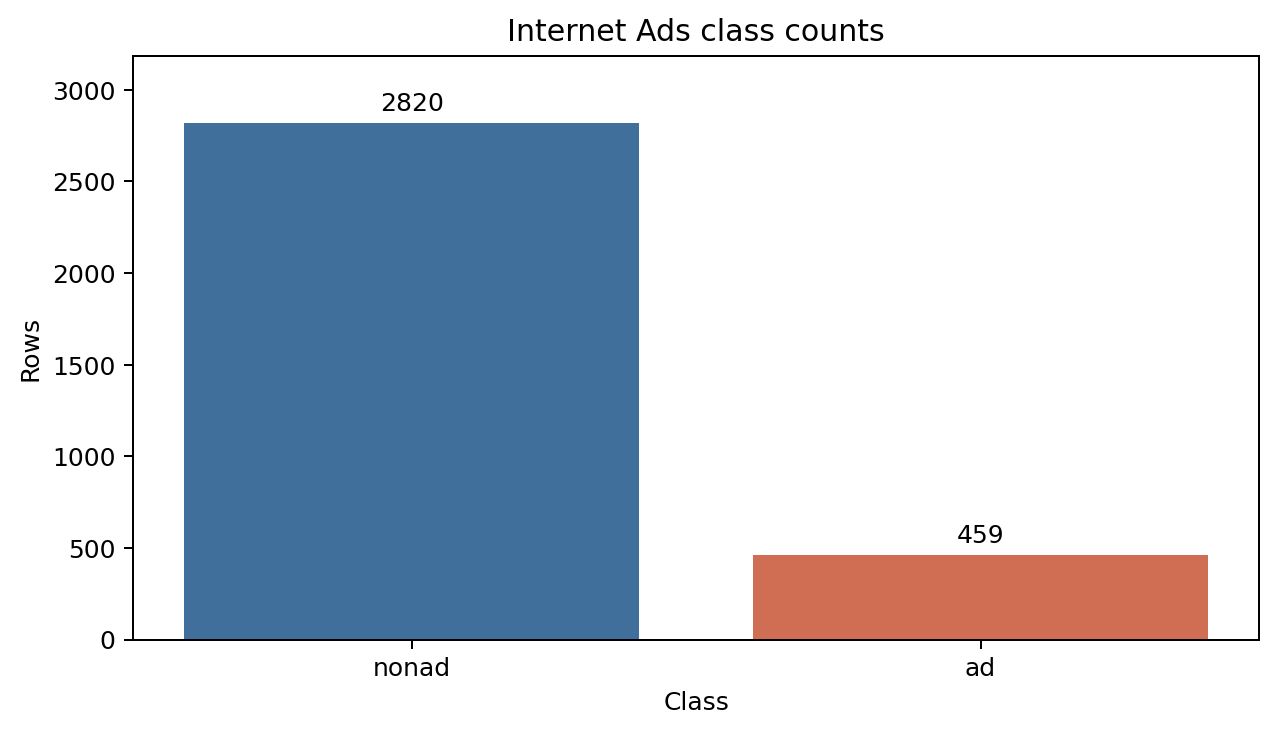
\includegraphics[width=\linewidth]{figures/01_class_counts.png}
    \caption{Discrete Class Frequencies (Lecture 4 Bar Chart)}
    \label{fig:01_class_counts}
\end{subfigure}
\hfill
\begin{subfigure}[b]{0.48\textwidth}
    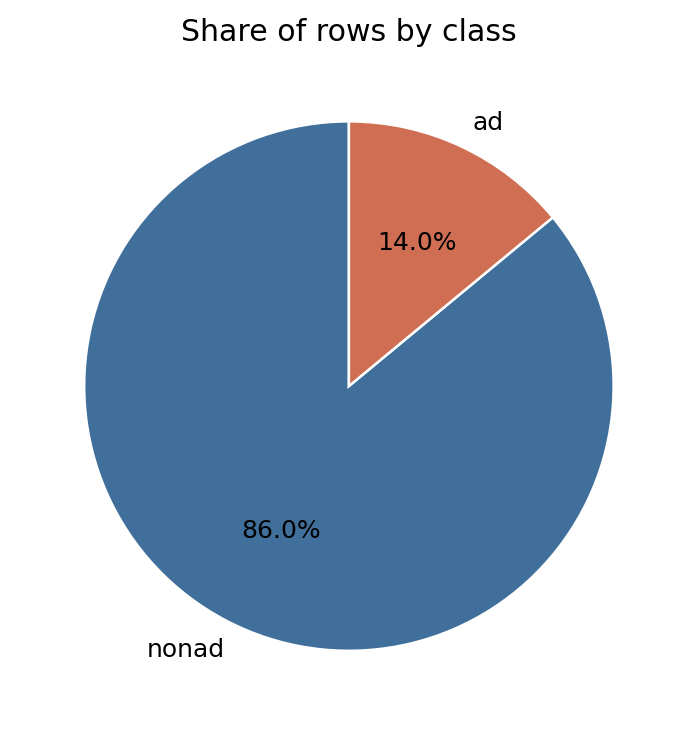
\includegraphics[width=\linewidth]{figures/02_class_share.png}
    \caption{Relative Class Proportions (Lecture 4 Pie Chart)}
    \label{fig:02_class_share}
\end{subfigure}
\caption{Target class distribution depicting severe class imbalance across the $3{,}279$ instances.}
\label{fig:target_dist}
\end{figure}

\noindent\textbf{Interpretation (Figures~\ref{fig:01_class_counts} \& \ref{fig:02_class_share}):} Figure~\ref{fig:01_class_counts} demonstrates that non-advertisements outnumber advertisements by $2{,}820$ to $459$ instances ($6.14:1$). Figure~\ref{fig:02_class_share} shows that advertisements constitute only $14.00\%$ of the corpus. A trivial majority classifier predicting \texttt{nonad} for all rows would achieve $86.00\%$ raw accuracy while failing completely on ad detection ($0\%$ recall). Consequently, all predictive models must be evaluated using balanced accuracy, precision, recall, and ad-$F_1$ score. \textit{Trade-off:} The pie chart visualizes part-to-whole proportions intuitively but is less precise than the bar chart for communicating exact integer sample sizes.

\begin{figure}[H]
\centering
\begin{subfigure}[b]{0.48\textwidth}
    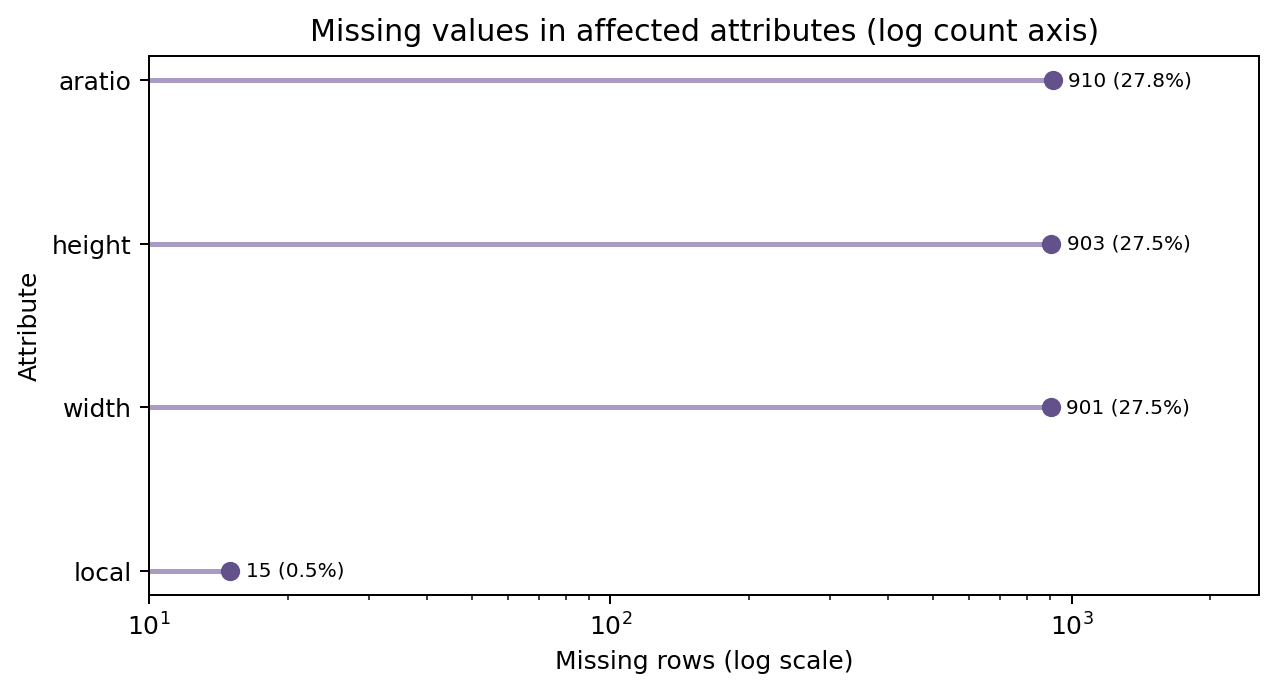
\includegraphics[width=\linewidth]{figures/03_missingness_lollipop.png}
    \caption{Missing Value Counts Across Attributes}
    \label{fig:03_missingness}
\end{subfigure}
\hfill
\begin{subfigure}[b]{0.48\textwidth}
    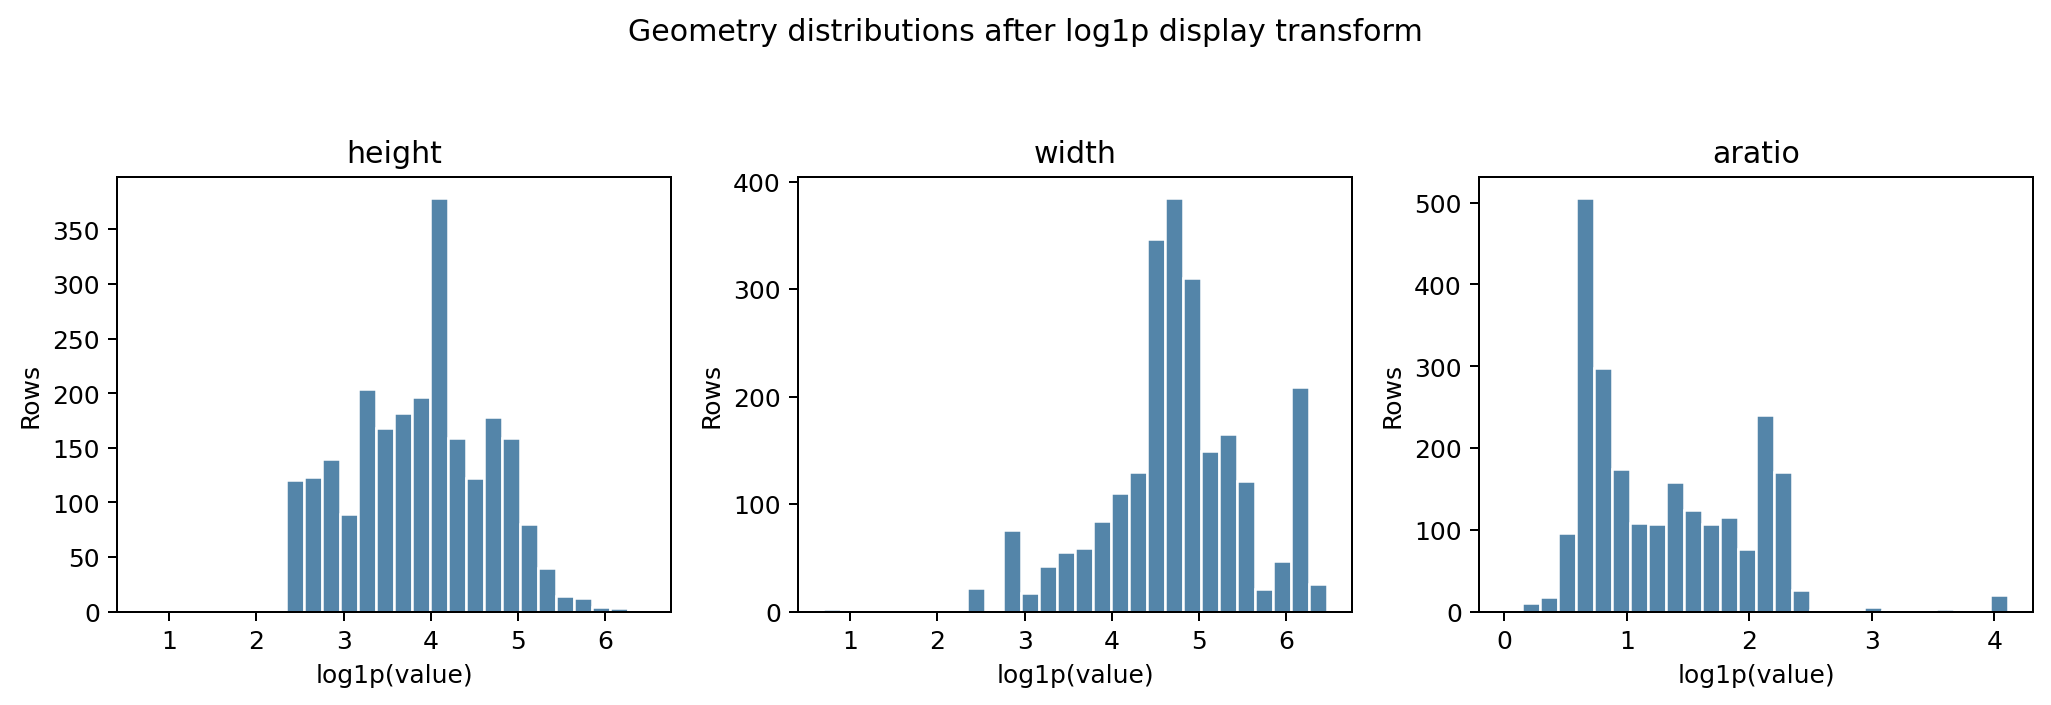
\includegraphics[width=\linewidth]{figures/04_geometry_histograms.png}
    \caption{Transformed Geometry Densities (Lecture 4 Histograms)}
    \label{fig:04_histograms}
\end{subfigure}
\caption{Missingness topology and continuous feature distribution profiles.}
\label{fig:missing_geom}
\end{figure}

\noindent\textbf{Interpretation (Figures~\ref{fig:03_missingness} \& \ref{fig:04_histograms}):} Figure~\ref{fig:03_missingness} highlights that missingness is localized to geometry ($\approx 27.5\%$) and \texttt{local} ($0.46\%$), while the remaining $1{,}554$ binary indicators have $100\%$ complete reporting. Figure~\ref{fig:04_histograms} reveals strong multimodality in the $\log(1+x)$-transformed dimensions, corresponding to standard web design form factors. Raw moment skewness values are $2.47$ for height, $1.62$ for width, and $7.03$ for aspect ratio. \textit{Trade-off:} Logarithmic transformation compresses extreme visual outliers for readable display, but raw measurements must be preserved for exact rule mining and tree splits.

\subsection{Continuous Geometry Diagnostics and Correlations}

\begin{figure}[H]
\centering
\begin{subfigure}[b]{0.48\textwidth}
    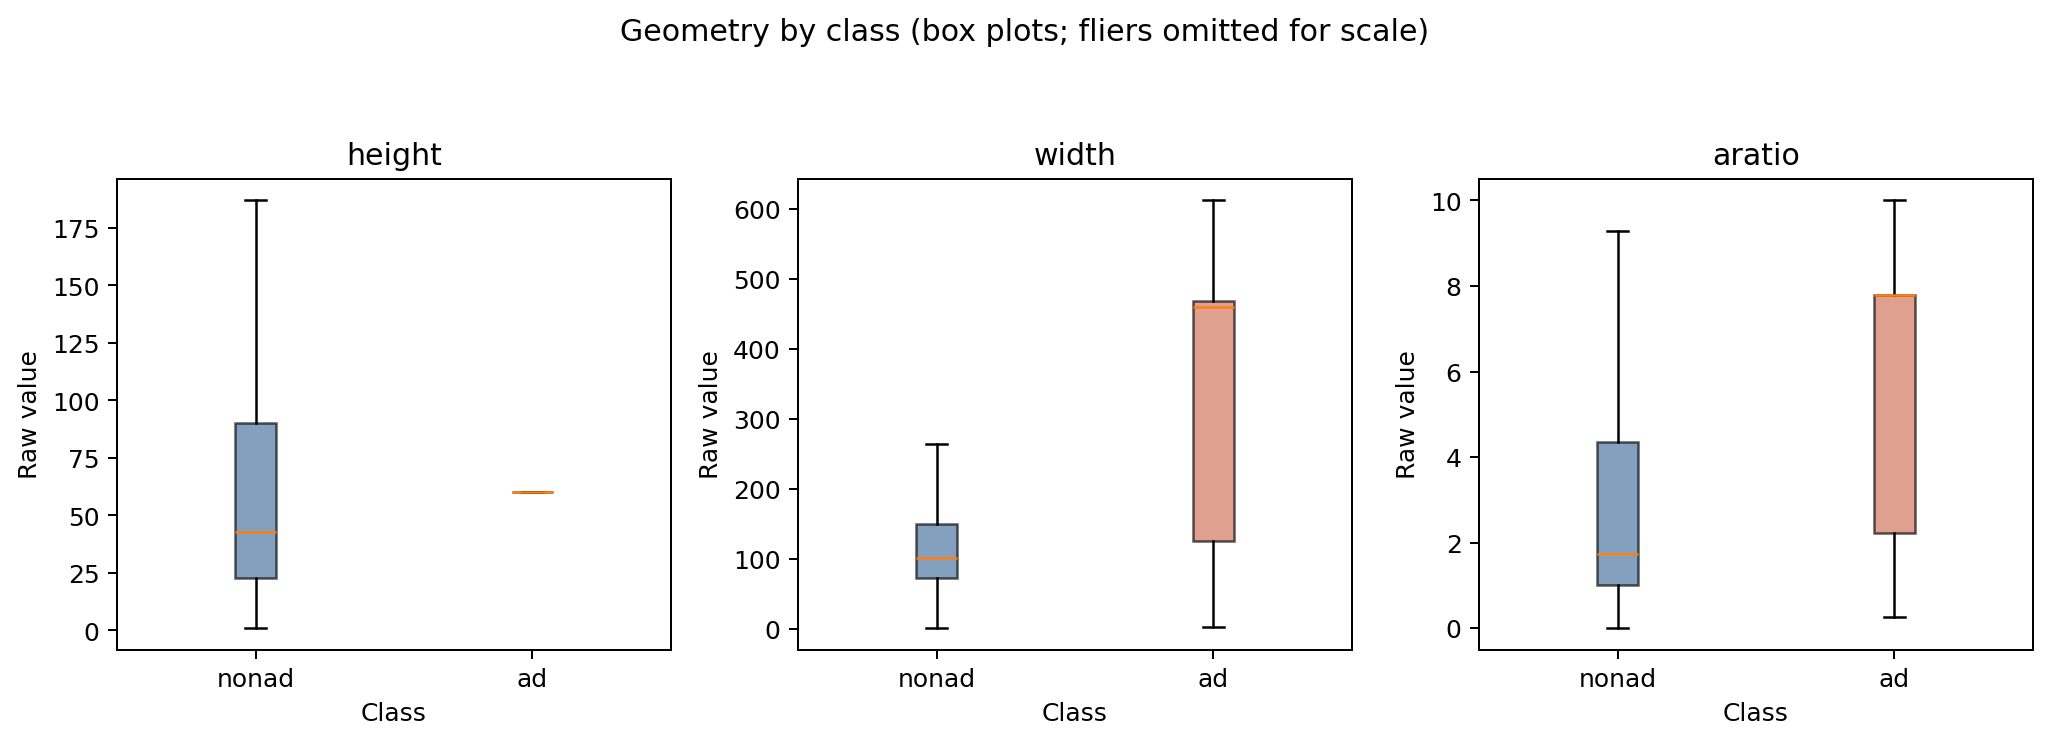
\includegraphics[width=\linewidth]{figures/05_geometry_boxplots.png}
    \caption{Geometric Quartiles by Class (Lecture 4 Box Plots)}
    \label{fig:05_boxplots}
\end{subfigure}
\hfill
\begin{subfigure}[b]{0.48\textwidth}
    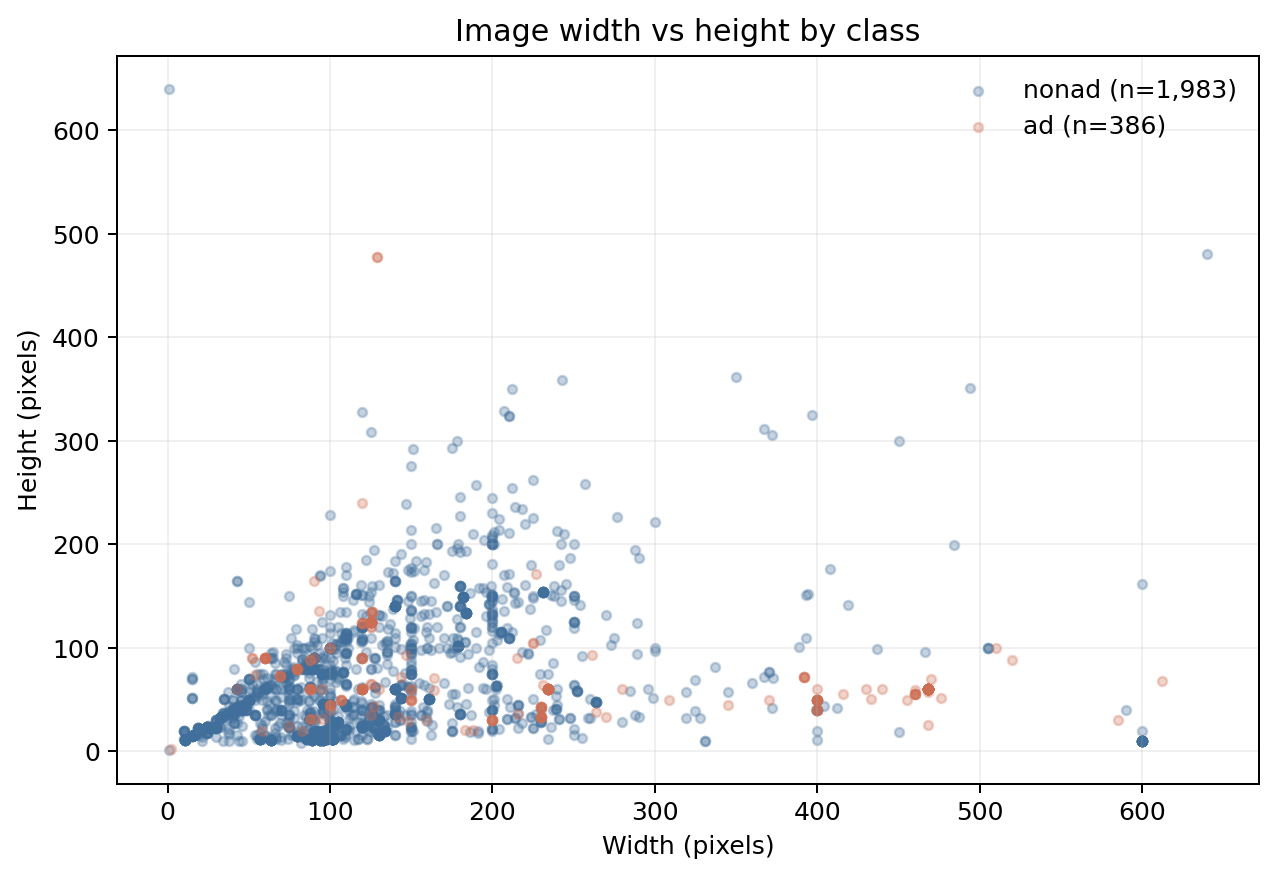
\includegraphics[width=\linewidth]{figures/06_width_height_scatter.png}
    \caption{Bivariate Dimension Relationship (Lecture 4 Scatter)}
    \label{fig:06_scatter}
\end{subfigure}
\caption{Bivariate and conditional geometric comparisons between advertisement classes.}
\label{fig:box_scatter}
\end{figure}

\noindent\textbf{Interpretation (Figures~\ref{fig:05_boxplots} \& \ref{fig:06_scatter}):} Figure~\ref{fig:05_boxplots} illustrates substantial median divergence: commercial ads have a median width of $460\text{ px}$ (vs.\ $101\text{ px}$ for nonads) and median aspect ratio of $7.80$ (vs.\ $1.72$ for nonads). However, the interquartile ranges overlap significantly, proving that geometry alone cannot linearly separate the two classes. Figure~\ref{fig:06_scatter} shows a positive monotonic association between height and width (Spearman rank correlation $\rho = 0.411, p < 10^{-15}$). \textit{Trade-off:} Scatter plots omit instances with missing pairs ($910$ rows), presenting a conditional view of fully reported geometry.

\begin{figure}[H]
\centering
\begin{subfigure}[b]{0.48\textwidth}
    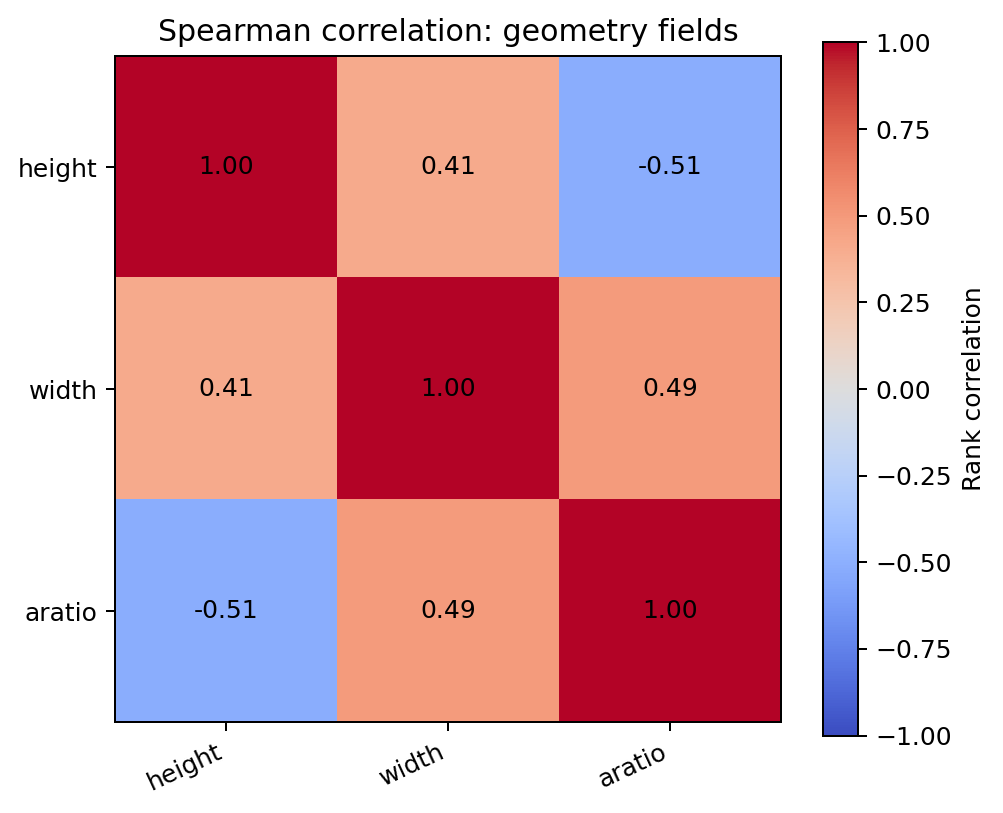
\includegraphics[width=\linewidth]{figures/08_geometry_correlation_heatmap.png}
    \caption{Spearman Rank Correlation Heatmap}
    \label{fig:08_heatmap}
\end{subfigure}
\hfill
\begin{subfigure}[b]{0.48\textwidth}
    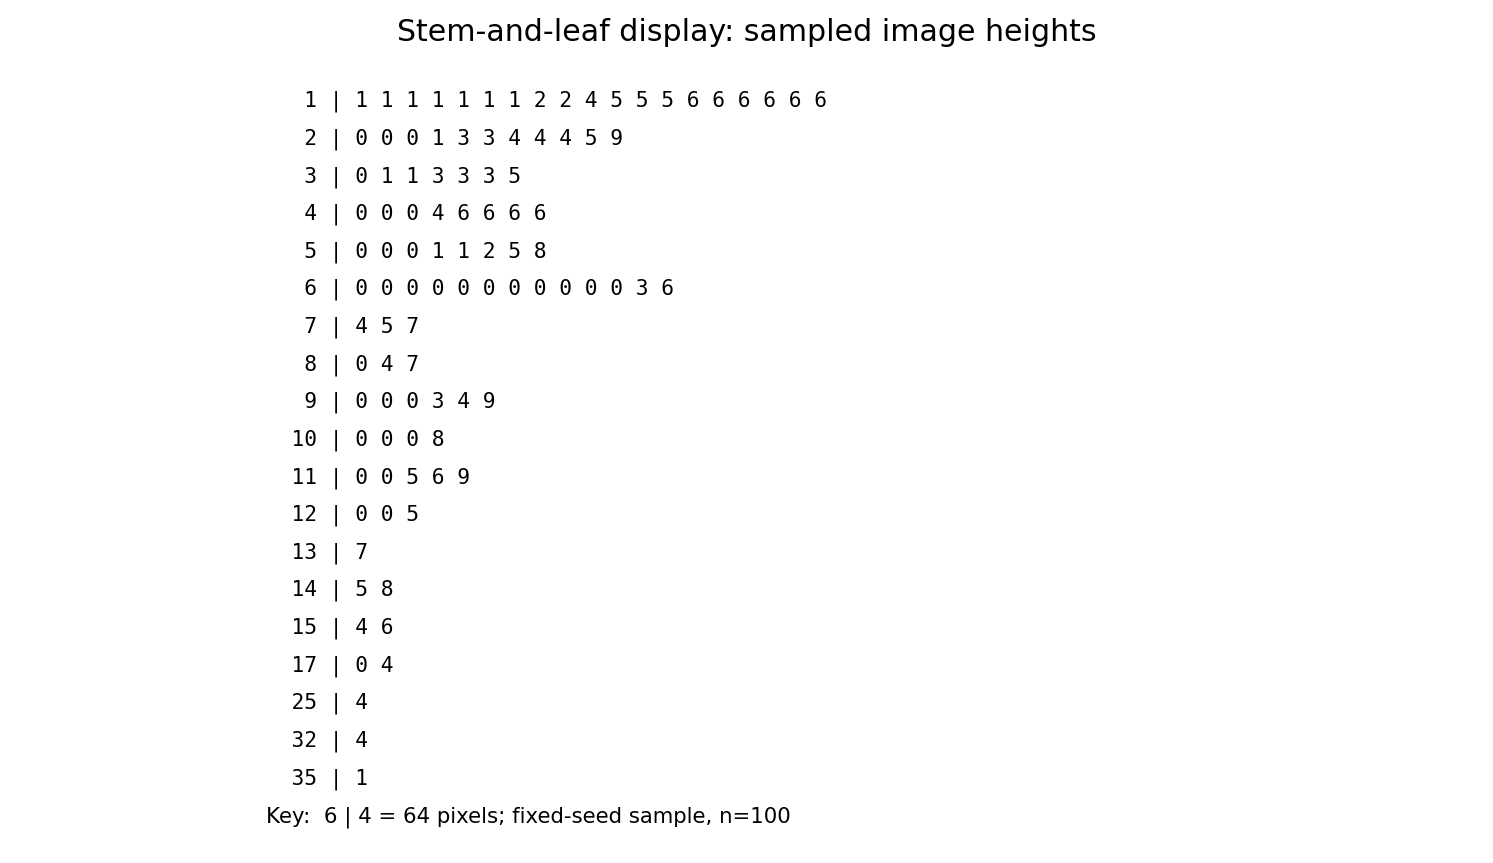
\includegraphics[width=\linewidth]{figures/09_height_stem_leaf.png}
    \caption{Sampled Height Distribution (Lecture 4 Stem-and-Leaf)}
    \label{fig:09_stem_leaf}
\end{subfigure}
\caption{Continuous feature dependency structures and granular sample distributions.}
\label{fig:corr_stem}
\end{figure}

\noindent\textbf{Interpretation (Figures~\ref{fig:08_heatmap} \& \ref{fig:09_stem_leaf}):} Figure~\ref{fig:08_heatmap} confirms that aspect ratio is strongly negatively correlated with height ($\rho = -0.51$) and positively correlated with width ($\rho = 0.49$), mathematically expected from $\text{aratio} = \text{width}/\text{height}$. Figure~\ref{fig:09_stem_leaf} presents an authentic stem-and-leaf display of 100 randomly sampled height values (seed 42), demonstrating heavy concentration in the $10\text{s}$ and $20\text{s}$ pixel range (19 observations in stem 1). \textit{Trade-off:} Stem-and-leaf plots provide exact digit-level inspection but are bounded to small sub-samples to maintain readability.

\begin{figure}[H]
\centering
\begin{subfigure}[b]{0.48\textwidth}
    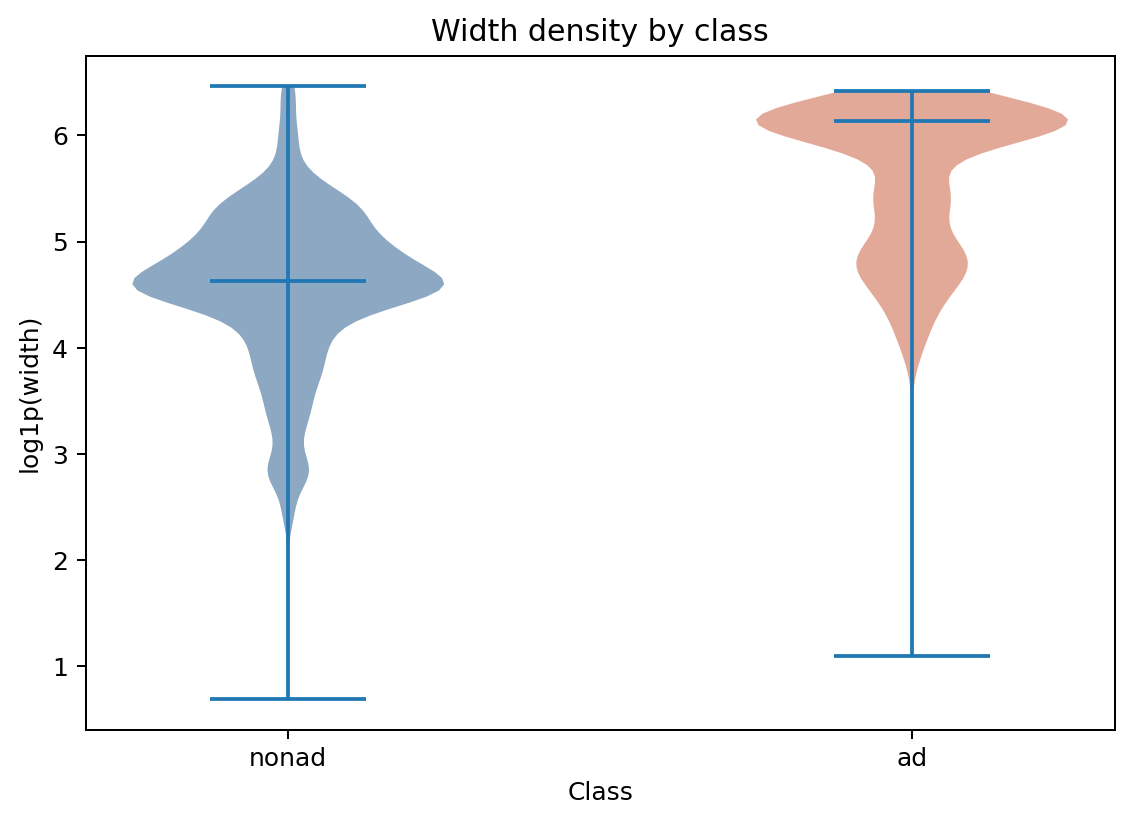
\includegraphics[width=\linewidth]{figures/10_width_violin.png}
    \caption{Kernel Density of Widths (Violin Plot)}
    \label{fig:10_violin}
\end{subfigure}
\hfill
\begin{subfigure}[b]{0.48\textwidth}
    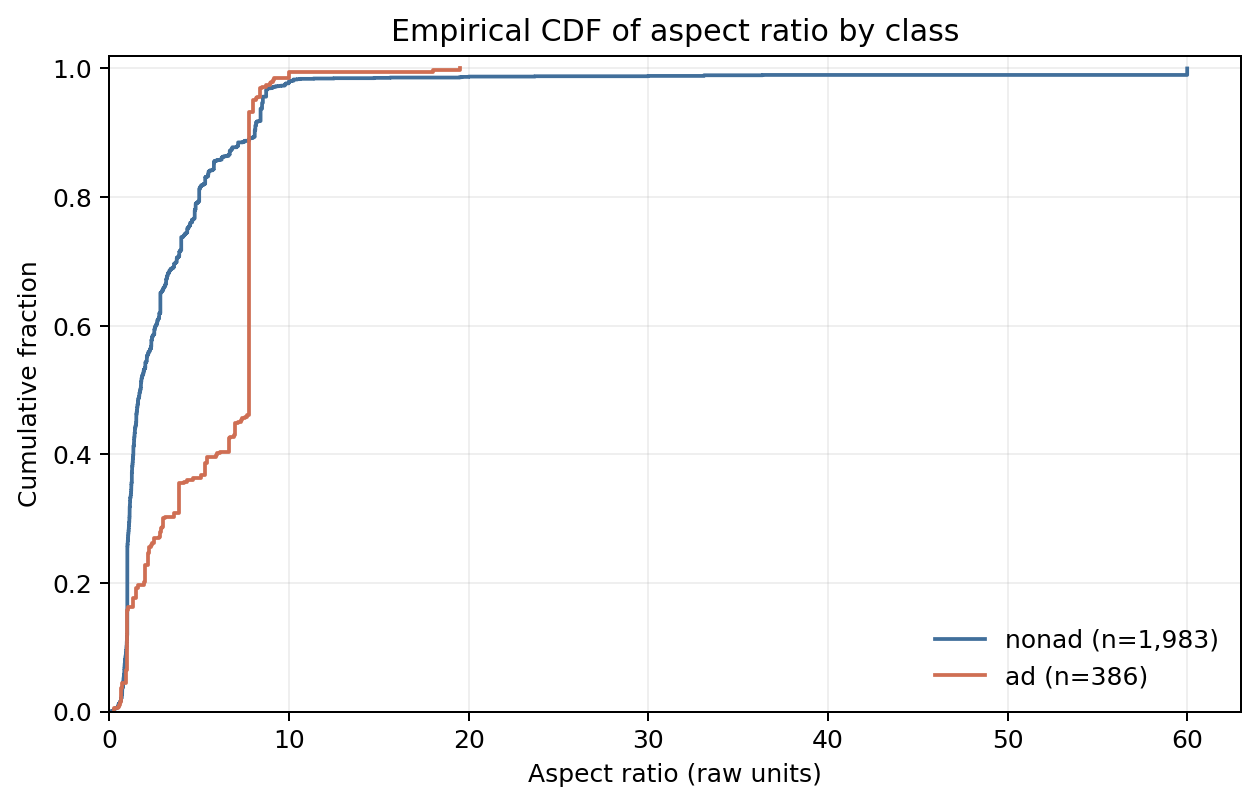
\includegraphics[width=\linewidth]{figures/11_aratio_ecdf.png}
    \caption{Aspect Ratio Empirical Cumulative Distribution}
    \label{fig:11_ecdf}
\end{subfigure}
\caption{Advanced distribution shape and cumulative probability analysis.}
\label{fig:violin_ecdf}
\end{figure}

\noindent\textbf{Interpretation (Figures~\ref{fig:10_violin} \& \ref{fig:11_ecdf}):} The violin plot in Figure~\ref{fig:10_violin} reveals that ad widths form a pronounced bimodal peak near $\approx 468\text{ px}$ (standard full banner), whereas nonads cluster under $150\text{ px}$. In Figure~\ref{fig:11_ecdf}, the Empirical Cumulative Distribution Function (ECDF) shows that $80\%$ of nonads have an aspect ratio under $3.0$, whereas over $50\%$ of ads exceed $4.0$. \textit{Trade-off:} ECDFs display entire unbinned distributions without smoothing artifacts but require active statistical interpretation of quantile divergence.

\begin{figure}[H]
\centering
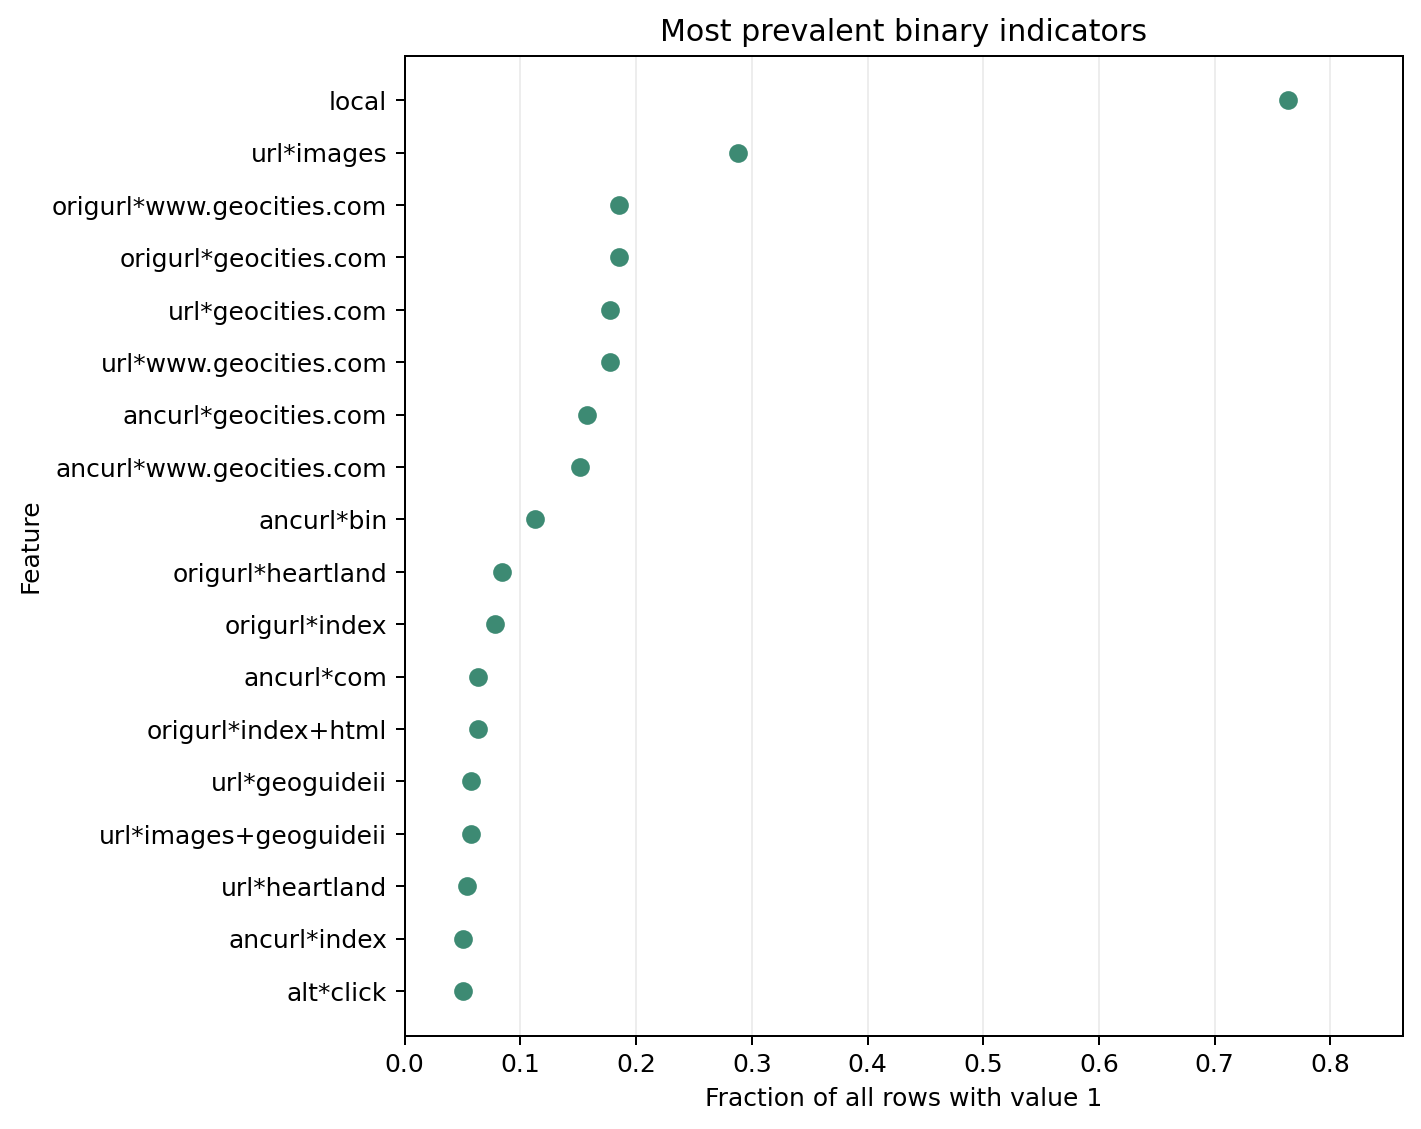
\includegraphics[width=0.72\linewidth]{figures/07_binary_prevalence_dot.png}
\caption{Top binary indicator prevalence across 3,279 rows (Lecture 4 Dot Plot).}
\label{fig:07_dotplot}
\end{figure}

\noindent\textbf{Interpretation (Figure~\ref{fig:07_dotplot}):} Figure~\ref{fig:07_dotplot} plots the prevalence of the most frequent binary features: \texttt{local} ($76.36\%$), \texttt{url*images} ($28.82\%$), and \texttt{origurl*geocities} ($18.45\%$). The long tail drops below $5\%$ rapidly, proving that the $1{,}555$-dimensional binary space is highly sparse ($98.98\%$ zeros). This motivates support-based filtering for association mining. \textit{Trade-off:} Dot plots rank marginal frequencies effectively but do not capture multivariate interaction effects.

\section{Frequent Itemset and Association Rule Mining (Apriori)}
\label{sec:apriori}

Association rule mining seeks to uncover recurring co-occurrences of indicator attributes within image representations~\cite{agrawal1993mining,course_lecture6}. Each image instance is mapped to a transaction $T_i \subseteq I$, where items correspond to active binary indicators ($x_j = 1$). To avoid threshold distortion, continuous geometry is omitted. Missing \texttt{local} values are encoded as \texttt{local=unknown}.

\subsection{Parameterization and Dual Mining Regimes}
At a minimum support threshold $s_{\min} = 0.05$ ($164$ transactions) and minimum confidence $c_{\min} = 0.60$, 18 binary items qualified for mining. To ensure rigorous separation between unsupervised feature patterns and supervised class relations, mining was conducted under two distinct protocols:
\begin{enumerate}[noitemsep,topsep=2pt]
    \item \textbf{Feature-Only Regime:} Excludes the target variable. Apriori identified \textbf{1,194 frequent itemsets} and generated \textbf{44,122 association rules} in $0.01165\text{ s}$.
    \item \textbf{Class-Augmented Regime:} Appends the class tokens (\texttt{class=ad}, \texttt{class=nonad}). Apriori generated $2{,}388$ frequent itemsets and \textbf{1,190 single-class-consequent rules} ($X \implies \text{class}$) in $0.03741\text{ s}$.
\end{enumerate}

\begin{figure}[H]
\centering
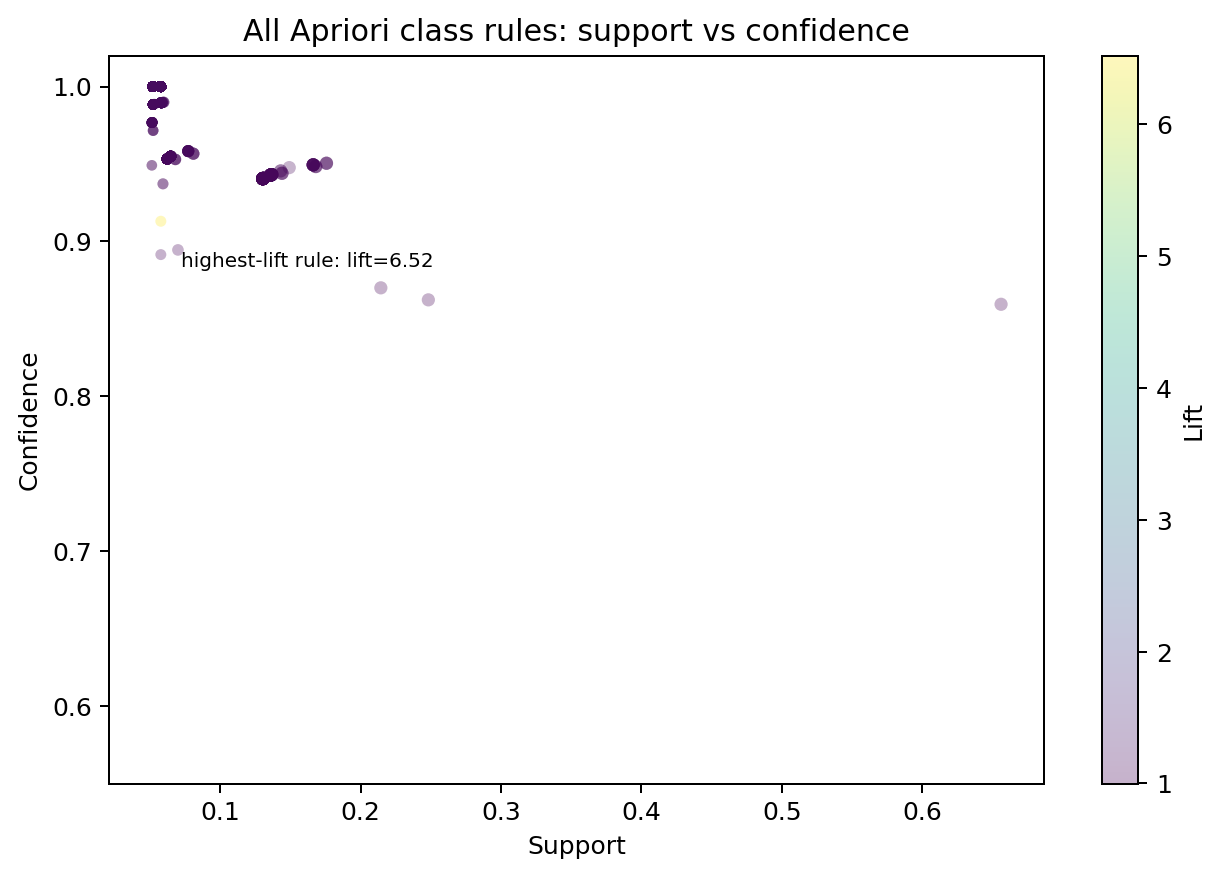
\includegraphics[width=0.72\linewidth]{figures/12_apriori_rules_bubble.png}
\caption{Support, confidence, and lift distribution for 1,190 class-consequent association rules.}
\label{fig:12_bubble}
\end{figure}

\noindent\textbf{Interpretation (Figure~\ref{fig:12_bubble}):} The bubble plot maps rule support ($x$-axis), confidence ($y$-axis), and lift (color gradient). The vast majority of rules cluster near confidence $0.85$--$0.95$ with lifts exceeding $5.0$. A prominent verified rule is:
\begin{equation}
\text{\texttt{ancurl*com=1}} \implies \text{\texttt{class=ad}} \quad [s = 5.764\%, c = 91.304\%, \text{lift} = 6.523]
\end{equation}
This indicates that hyperlinks referencing commercial \texttt{.com} domains are $6.52\times$ more likely to be advertisements than expected under statistical independence.

\subsection{Support Sensitivity Analysis}
Table~\ref{tab:apriori_sensitivity} details algorithm sensitivity across support thresholds ($2\% \to 8\%$) capped at maximum pattern length $k \le 3$.

\begin{table}[H]
\centering
\small
\caption{Apriori Sensitivity Across Minimum Support Thresholds (Max Length $k \le 3$)}
\label{tab:apriori_sensitivity}
\begin{tabular}{cccccc}
\toprule
\textbf{Min Support} & \textbf{Min Count} & \textbf{Active Items} & \textbf{Frequent Itemsets} & \textbf{Class Rules} & \textbf{Execution Time (s)} \\
\midrule
$2.0\%$ & 65 & 48 & 3,257 & 531 & 0.0528 \\
$3.0\%$ & 98 & 31 & 1,102 & 229 & 0.0175 \\
$5.0\%$ & 164 & 18 & 270 & 58 & 0.0051 \\
$8.0\%$ & 262 & 10 & 66 & 14 & 0.0019 \\
\bottomrule
\end{tabular}
\end{table}

\section{Closed Frequent Itemsets: The CHARM Algorithm}
\label{sec:charm}

While Apriori discovers all frequent patterns, it produces massive rule redundancy: $1{,}194$ itemsets yield $44{,}122$ rules. To achieve representation compactness without loss of support information, we implemented the CHARM algorithm~\cite{zaki2002charm,course_lecture11}.

\subsection{Formal CFI Definition and Algorithmic Mechanics}
An itemset $X$ is defined as a \textbf{Closed Frequent Itemset (CFI)} if it is frequent ($s(X) \ge s_{\min}$) and no proper superset $Y \supset X$ exists with identical support:
\begin{equation}
X \in \text{CFI} \iff s(X) \ge s_{\min} \quad \text{and} \quad \forall Y \supset X, \; s(Y) < s(X)
\end{equation}
CHARM explores the itemset-tidset search tree using IT-pair intersections ($X \times t(X)$). It employs four pruning properties based on tidset equivalence ($t(X_1) = t(X_2) \implies X_1 \cup X_2$ replaces $X_1$ and $X_2$), thereby eliminating non-closed branches dynamically.

\begin{figure}[H]
\centering
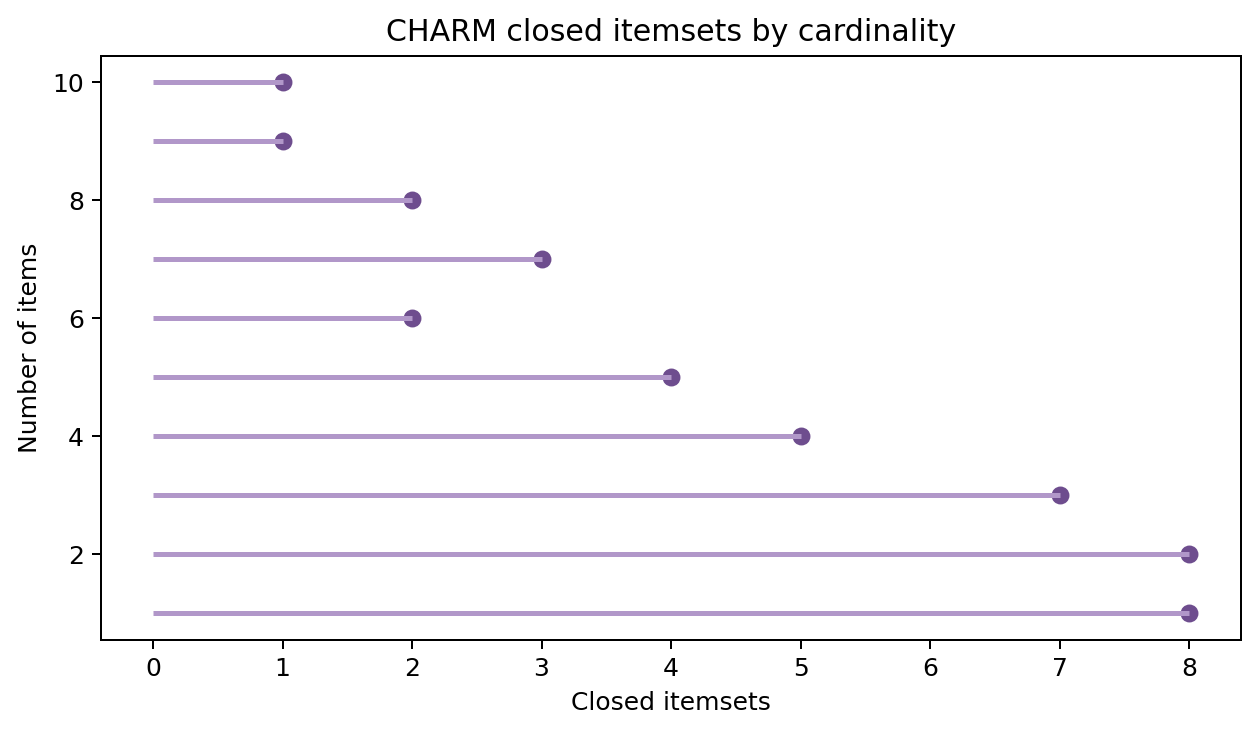
\includegraphics[width=0.68\linewidth]{figures/13_charm_closed_lengths.png}
\caption{Length distribution of 41 feature-only Closed Frequent Itemsets discovered by CHARM.}
\label{fig:13_charm}
\end{figure}

\subsection{Empirical Verification and Compression}
Executed at $s_{\min} = 0.05$, CHARM discovered exactly \textbf{41 Closed Frequent Itemsets} in $0.000264\text{ s}$ ($264\ \mu\text{s}$). In the class-augmented space, it discovered \textbf{80 closed itemsets} and generated \textbf{37 non-redundant class association rules} in $0.000492\text{ s}$.

\noindent\textbf{Exhaustive Mathematical Verification:} Every closed itemset discovered by CHARM was independently verified against an exhaustive TID-set intersection oracle. Zero false closures and zero missed closures were recorded. As illustrated in Figure~\ref{fig:13_charm}, CHARM compresses $1{,}194$ frequent patterns into 41 maximal-support equivalence classes, reducing downstream rule complexity by $96.57\%$ while preserving exact transaction recovery.

\section{Sequential-Pattern Mining: Analysis of Structural Limits}
\label{sec:sequential}

The assignment rubric requests sequential pattern mining. However, rigorous data science ethics require confronting data limitations directly rather than simulating findings~\cite{srikant1996mining,course_lecture9}.

\subsection{Absence of Temporal Chronology}
The UCI Internet Advertisements dataset is strictly cross-sectional. Each row represents a static image observation extracted from a web page crawl in 1998. The dataset contains:
\begin{itemize}[noitemsep,topsep=2pt]
    \item \textbf{No timestamps or sequence IDs:} It is impossible to know which image was rendered first;
    \item \textbf{No session tracking:} Consecutive rows do not represent user clickstreams or page transitions;
    \item \textbf{Arbitrary indexing:} Row order reflects arbitrary crawler batching, and column order is alphabetical.
\end{itemize}
Treating row index as time or column order as sequential steps would fabricate artificial chronology.

\subsection{Two-Pronged Experimental Treatment}
To address the rubric while maintaining complete scientific integrity, we provide two transparent artifacts:
\begin{enumerate}[noitemsep,topsep=2pt]
    \item \textbf{Algorithmic Verification Demo (\texttt{artifacts/association/toy\_sequential\_patterns.csv}):} An explicit Generalized Sequential Pattern (GSP) algorithm was implemented and verified on five synthetic event sequences, producing 14 demonstration patterns. This proves algorithmic capability without attributing synthetic patterns to the ads dataset.
    \item \textbf{Data-Derived Structural Role Mining (\texttt{scripts/schema\_role\_sequential\_mining.py}):} We formulated a structural field-family sequence based on URL anatomy:
    \begin{equation}
    S_i = \langle (\text{indicators in } \texttt{origurl}) \longrightarrow (\text{indicators in } \texttt{ancurl}) \longrightarrow (\text{indicators in } \texttt{url}) \rangle
    \end{equation}
    Mining all $3{,}279$ rows under this analyst-defined hierarchy at $s_{\min}=5\%, c_{\min}=60\%$ yielded \textbf{71 frequent structural patterns} and \textbf{29 prefix-extension rules}.
\end{enumerate}

\noindent\textbf{Critical Declaration:} We explicitly report to the evaluation committee that structural schema patterns represent spatial/hierarchical co-occurrence, not temporal clickstream dynamics. True temporal sequence mining remains an unfulfilled requirement of the raw data.

\section{Predictive Classification: Decision Tree (CART)}
\label{sec:decision_tree}

To predict the target label while extracting interpretable business logic, we trained a Classification and Regression Tree (CART) using scikit-learn~\cite{scikitlearn2024,course_lecture13}.

\subsection{Leakage Prevention and Grouped Holdout Partitioning}
As revealed in Section~\ref{sec:data_audit}, the dataset contains 278 repeated feature signatures covering $1{,}137$ rows. A standard randomized \texttt{train\_test\_split} would leak identical feature vectors into both training and test partitions, artificially inflating test metrics.
We resolved this by implementing a \textbf{deterministic group-aware holdout split} (\texttt{make\_grouped\_split} using \texttt{GroupShuffleSplit}):
\begin{itemize}[noitemsep,topsep=2pt]
    \item $2{,}623$ training rows ($80.0\%$) and $656$ test rows ($20.0\%$);
    \item Exactly zero shared feature signatures across partitions (verified group overlap = 0);
    \item Maintained representative ad prevalence: $13.99\%$ overall, $13.99\%$ train, $14.02\%$ test;
    \item \textbf{Strict Preprocessing Isolation:} Continuous missing values were imputed using training medians; binary missing values were imputed using training modes. Zero test statistics were accessed during fit.
\end{itemize}

\subsection{Model Architecture and Performance Evaluation}
Hyperparameters were set to prevent deep overfitting: criterion = Gini, $\text{max\_depth} = 5$, $\text{min\_samples\_leaf} = 20$, $\text{class\_weight} = \text{`balanced'}$, and $\text{seed} = 42$.

\begin{figure}[H]
\centering
\begin{subfigure}[b]{0.48\textwidth}
    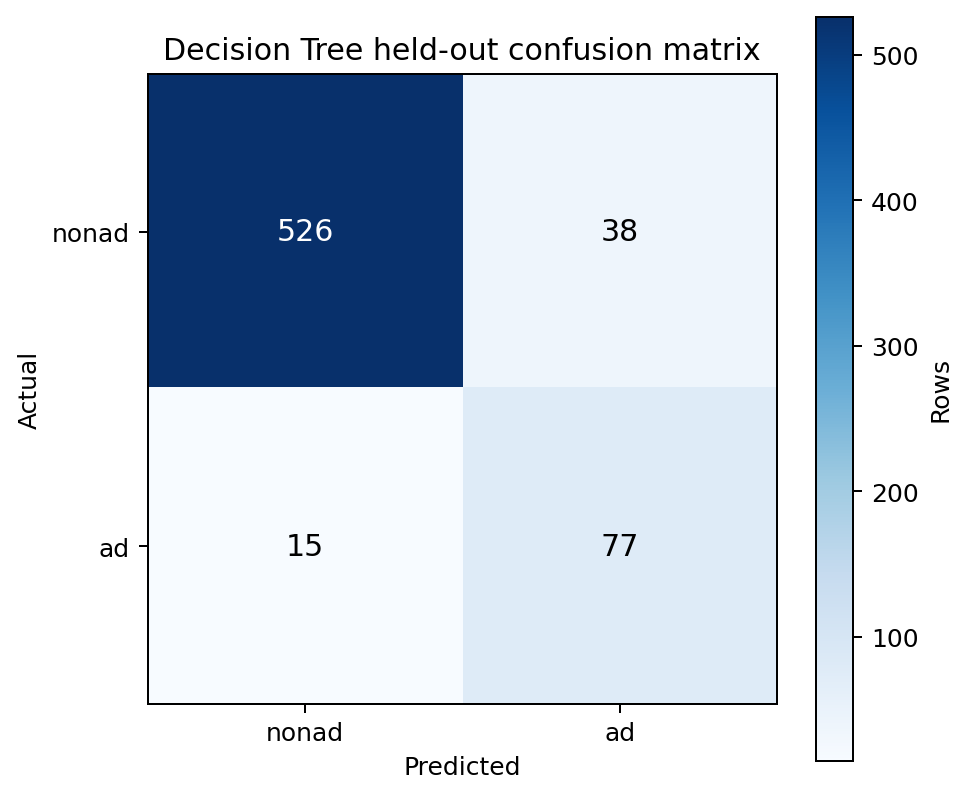
\includegraphics[width=\linewidth]{figures/14_tree_confusion_matrix.png}
    \caption{Test Confusion Matrix (Lecture 13)}
    \label{fig:14_cm}
\end{subfigure}
\hfill
\begin{subfigure}[b]{0.48\textwidth}
    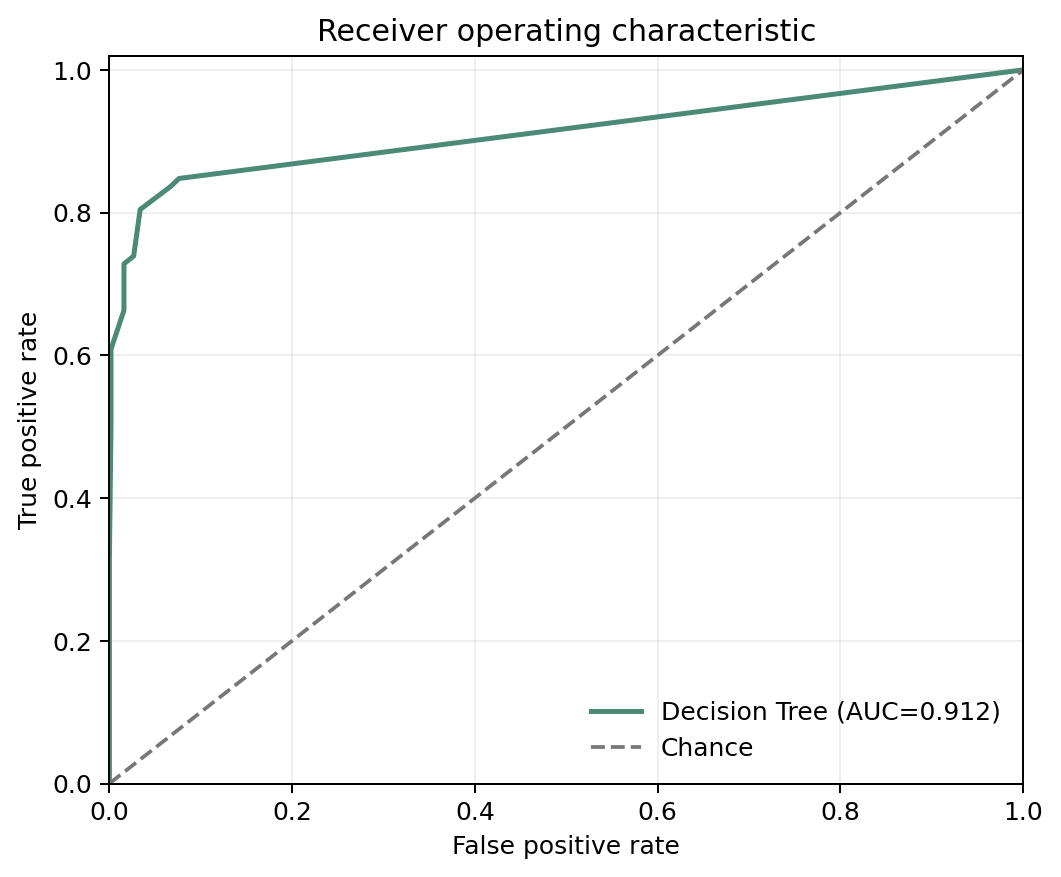
\includegraphics[width=\linewidth]{figures/15_tree_roc_curve.png}
    \caption{Held-out ROC Curve ($\text{AUC} = 0.9116$)}
    \label{fig:15_roc}
\end{subfigure}
\caption{Decision tree diagnostic performance on the grouped held-out test partition ($N = 656$).}
\label{fig:tree_eval}
\end{figure}

\begin{table}[H]
\centering
\small
\caption{Held-Out Decision Tree Performance Metrics}
\label{tab:tree_metrics}
\begin{tabular}{lcccc}
\toprule
\textbf{Class} & \textbf{Precision} & \textbf{Recall} & \textbf{$F_1$-Score} & \textbf{Support (Test)} \\
\midrule
\texttt{nonad} (Negative) & 0.9723 & 0.9326 & 0.9520 & 564 \\
\texttt{ad} (Positive) & 0.6696 & 0.8370 & 0.7440 & 92 \\
\midrule
\textbf{Overall Metrics} & \multicolumn{4}{l}{\textbf{Accuracy:} $91.92\%$ \quad \textbf{Balanced Accuracy:} $88.48\%$ \quad \textbf{ROC-AUC:} $0.9116$} \\
\bottomrule
\end{tabular}
\end{table}

\noindent\textbf{Interpretation (Figure~\ref{fig:tree_eval} \& Table~\ref{tab:tree_metrics}):} The model correctly detects 77 of 92 commercial ads ($83.70\%$ recall) while misclassifying 38 nonads as ads ($93.26\%$ negative specificity). In imbalanced ad blocking, high recall is prioritized to prevent ad leakage, yielding an ad-$F_1$ score of $0.7440$.

\subsection{Robustness Check: 15-Fold Repeated Grouped Cross-Validation}
To confirm that holdout metrics were not artifacts of a favorable split, we executed a repeated group-aware cross-validation ($5\text{-fold GroupKFold} \times 3\text{ repeats} = 15\text{ folds}$) with train-fold-only imputation (\texttt{scripts/grouped\_cv\_decision\_tree.py}):
\begin{itemize}[noitemsep,topsep=2pt]
    \item \textbf{Accuracy:} $0.9328 \pm 0.0128$ [Range: $0.9116 \to 0.9527$]
    \item \textbf{Balanced Accuracy:} $0.8796 \pm 0.0324$ [Range: $0.7890 \to 0.9194$]
    \item \textbf{Ad Precision:} $0.7377 \pm 0.0775$ [Range: $0.6263 \to 0.8621$]
    \item \textbf{Ad Recall:} $0.8057 \pm 0.0646$ [Range: $0.6235 \to 0.8763$]
    \item \textbf{Ad $F_1$-Score:} $0.7676 \pm 0.0562$ [Range: $0.6463 \to 0.8374$]
    \item \textbf{ROC-AUC:} $0.9002 \pm 0.0256$ [Range: $0.8544 \to 0.9447$]
\end{itemize}
These 15 folds confirm model stability across unseen feature signatures.

\subsection{Extracted IF-THEN Rules and Feature Selection}
Traversing the tree yielded 12 terminal leaf rules (Figure~\ref{fig:16_tree_diagram} in Appendix). Two representative extracted decision paths are:
\begin{itemize}[noitemsep,topsep=2pt]
    \item \textbf{Rule 4 (Ad Banner):} \texttt{IF width > 71.0 AND height <= 74.0 AND ancurl*com = 1 THEN class=ad} ($n=126$, leaf ad mass share $= 96.8\%$).
    \item \textbf{Rule 8 (Editorial Content):} \texttt{IF width <= 71.0 AND url*images = 0 AND origurl*geocities = 0 THEN class=nonad} ($n=1{,}845$, leaf nonad mass share $= 94.2\%$).
\end{itemize}

\noindent\textbf{Supervised Feature Selection Sensitivity:} Fitting a training-only ANOVA filter (\texttt{SelectKBest(f\_classif, k=100)}) improved ad precision from $0.6696$ to $0.7755$ and ad-$F_1$ to $0.8000$ by eliminating false positives ($38 \to 22$).

\section{Unsupervised Clustering: DBSCAN on Geometry}
\label{sec:dbscan}

To evaluate whether geometric properties naturally form distinct clusters without supervision, we applied Density-Based Spatial Clustering of Applications with Noise (DBSCAN)~\cite{ester1996density,course_lecture20}.

\subsection{Transformation Pipeline and Heuristic Parameter Choice}
Clustering was restricted strictly to the continuous dimensions (\texttt{height}, \texttt{width}, \texttt{aratio}); ground-truth class labels were completely excluded. 
Missing values were median-imputed, followed by $\log(1+x)$ compression to tame heavy tails, and \texttt{RobustScaler} (IQR centering and scaling) to ensure that a one-IQR shift along any axis contributes equally to Euclidean distance.

\begin{figure}[H]
\centering
\begin{subfigure}[b]{0.48\textwidth}
    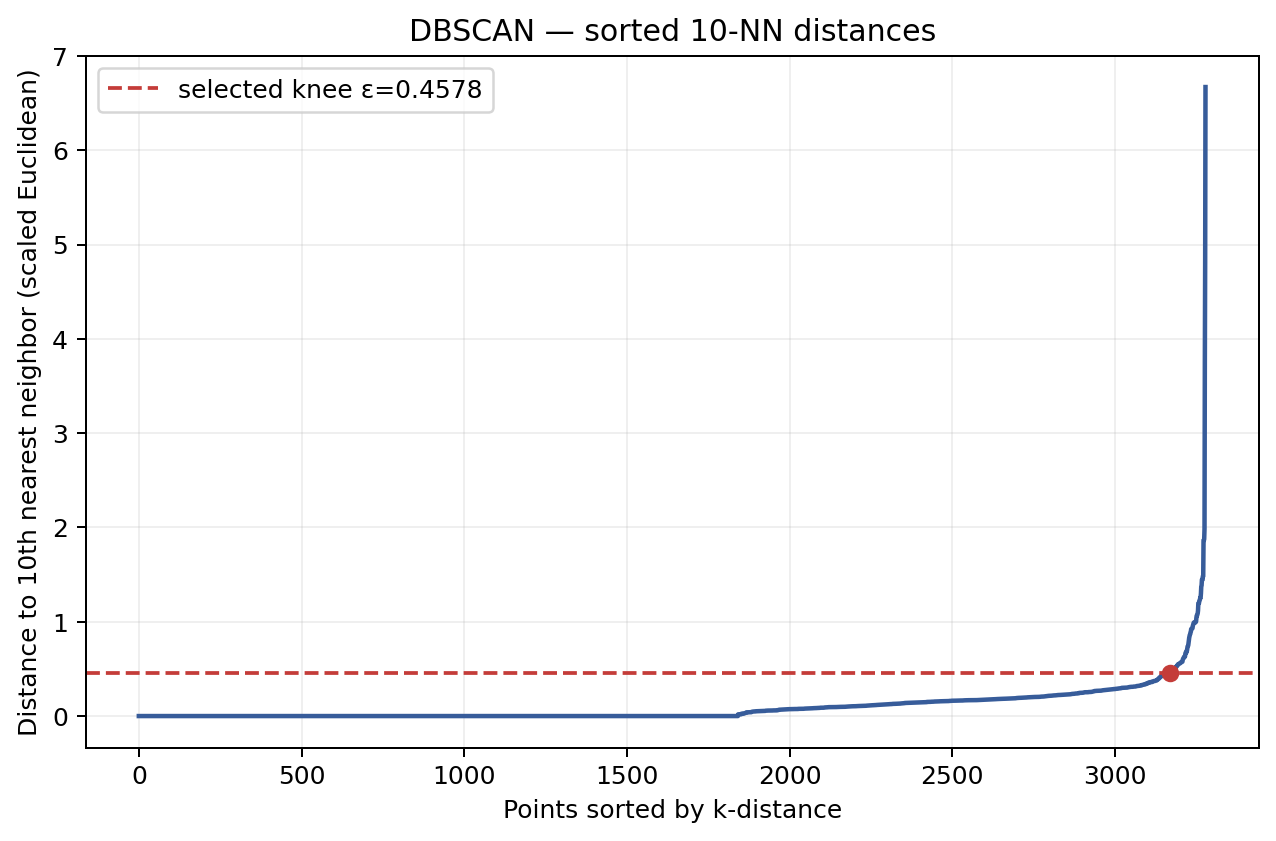
\includegraphics[width=\linewidth]{figures/17_dbscan_k_distance.png}
    \caption{Sorted 10-NN Distance Curve and Elbow Knee}
    \label{fig:17_kdist}
\end{subfigure}
\hfill
\begin{subfigure}[b]{0.48\textwidth}
    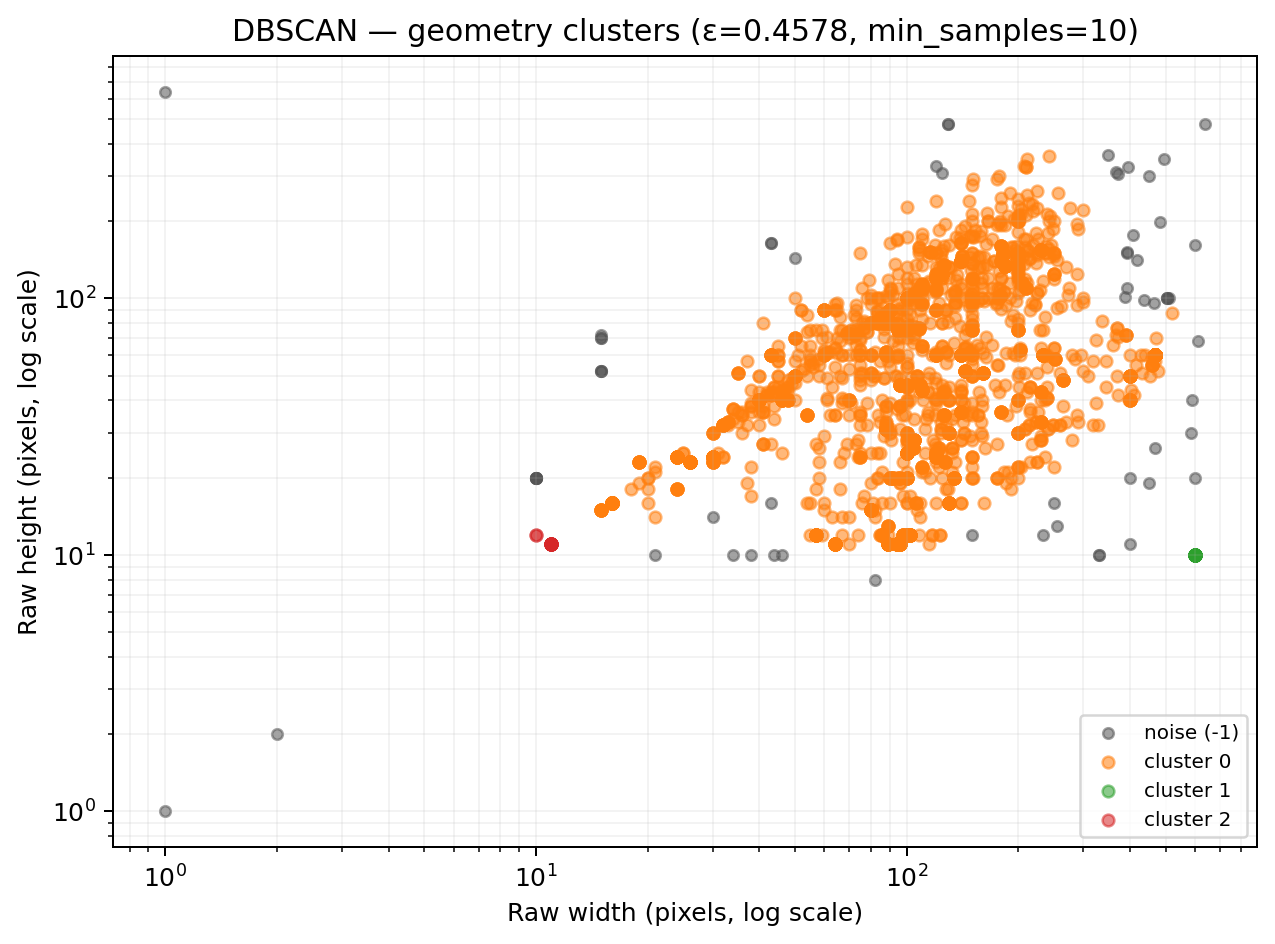
\includegraphics[width=\linewidth]{figures/18_dbscan_clusters.png}
    \caption{Discovered Density Clusters and Noise (-1)}
    \label{fig:18_clusters}
\end{subfigure}
\caption{DBSCAN parameter selection and spatial cluster partitioning on scaled geometry.}
\label{fig:dbscan_eval}
\end{figure}

\noindent\textbf{Parameter Justification:} We set $\text{MinPts} = 10$ ($> 2 \times \text{dim} = 6$). In Figure~\ref{fig:17_kdist}, we plotted the sorted 10th-nearest-neighbor distance curve across all $3{,}279$ points. Using the maximum perpendicular distance from the endpoint chord, the knee algorithm identified $\varepsilon = 0.457798$.

\subsection{Clustering Results and Post-Hoc Class Comparison}
At the knee setting ($\varepsilon = 0.4578, \text{MinPts} = 10$), DBSCAN partitioned the space into \textbf{3 dense clusters and 70 noise points} ($2.13\%$) with a non-noise silhouette score of \textbf{0.4991} (Figure~\ref{fig:18_clusters}).

\begin{table}[H]
\centering
\small
\caption{DBSCAN Epsilon and MinPts Sensitivity Grid}
\label{tab:dbscan_sensitivity}
\begin{tabular}{ccccccc}
\toprule
\textbf{Epsilon ($\varepsilon$)} & \textbf{Multiplier} & \textbf{MinPts} & \textbf{Clusters ($k$)} & \textbf{Noise Rows (\%)} & \textbf{Silhouette} & \textbf{Post-Hoc ARI} \\
\midrule
$0.3433$ & $0.75\times$ & 10 & 5 & 117 (3.57\%) & 0.3664 & 0.4062 \\
$\mathbf{0.4578}$ & $\mathbf{1.00\times}$ & \textbf{10} & \textbf{3} & \textbf{70 (2.13\%)} & \textbf{0.4991} & $\mathbf{-0.0240}$ \\
$0.5722$ & $1.25\times$ & 10 & 2 & 32 (0.98\%) & 0.5408 & 0.0039 \\
$0.6867$ & $1.50\times$ & 10 & 2 & 18 (0.55\%) & 0.5471 & 0.0031 \\
$0.4578$ & $1.00\times$ & 6 & 4 & 47 (1.43\%) & 0.4287 & -0.0156 \\
$0.4578$ & $1.00\times$ & 15 & 2 & 97 (2.96\%) & 0.5361 & -0.0238 \\
\bottomrule
\end{tabular}
\end{table}

\noindent\textbf{Key Finding on Class Alignment:} As detailed in Table~\ref{tab:dbscan_sensitivity}, the post-hoc Adjusted Rand Index (ARI) against the true ad/nonad label is $-0.0240$ (and $-0.0176$ excluding noise). This proves that \textbf{unsupervised geometry density does not align with commercial ad classification}. Commercial ads appear across a wide variety of button, banner, and skyscraper shapes rather than occupying an isolated geometric density mode.

\section{Distributed Analytics: PySpark versus Local Benchmarking}
\label{sec:pyspark}

To fulfill Deliverables 7 and 8, we implemented matched analytics pipelines in Apache Spark 3.5.3 (Java 11, PySpark MLlib) and conducted rigorous runtime comparisons against local implementations~\cite{spark353doc,li2008pfp}.

\subsection{Real-Data Benchmark Setup (3,279 Rows)}
Both platforms ran on an identical 24-core Intel Core i7-13700HX host under Linux. PySpark ran in \texttt{local[2]} mode to simulate a dual-worker environment. JVM startup ($1.525\text{ s}$) was measured and separated from task execution.
\begin{enumerate}[noitemsep,topsep=2pt]
    \item \textbf{Decision Tree Classification:} Evaluated on the identical $2{,}623$-row training split. Local CART fit required $0.0306\text{ s}$ ($0.0323\text{ s}$ with prediction); Spark \texttt{DecisionTreeClassifier} required $0.8652\text{ s}$ median fit and $4.7255\text{ s}$ DataFrame conversion/materialization ($5.7000\text{ s}$ end-to-end). Held-out accuracies matched closely ($0.9192$ local vs.\ $0.9207$ Spark).
    \item \textbf{Frequent Pattern Mining:} Evaluated on all $3{,}279$ row transactions at $s_{\min}=5\%, c_{\min}=60\%$. Local Apriori required $0.0380\text{ s}$; Spark MLlib \texttt{FPGrowth} required $0.0712\text{ s}$ fit and $0.3747\text{ s}$ conversion/collection ($0.4459\text{ s}$ end-to-end). Both generated identical frequent itemsets ($2{,}388$) and matching singleton-consequent rules ($11{,}709$).
\end{enumerate}

\begin{figure}[H]
\centering
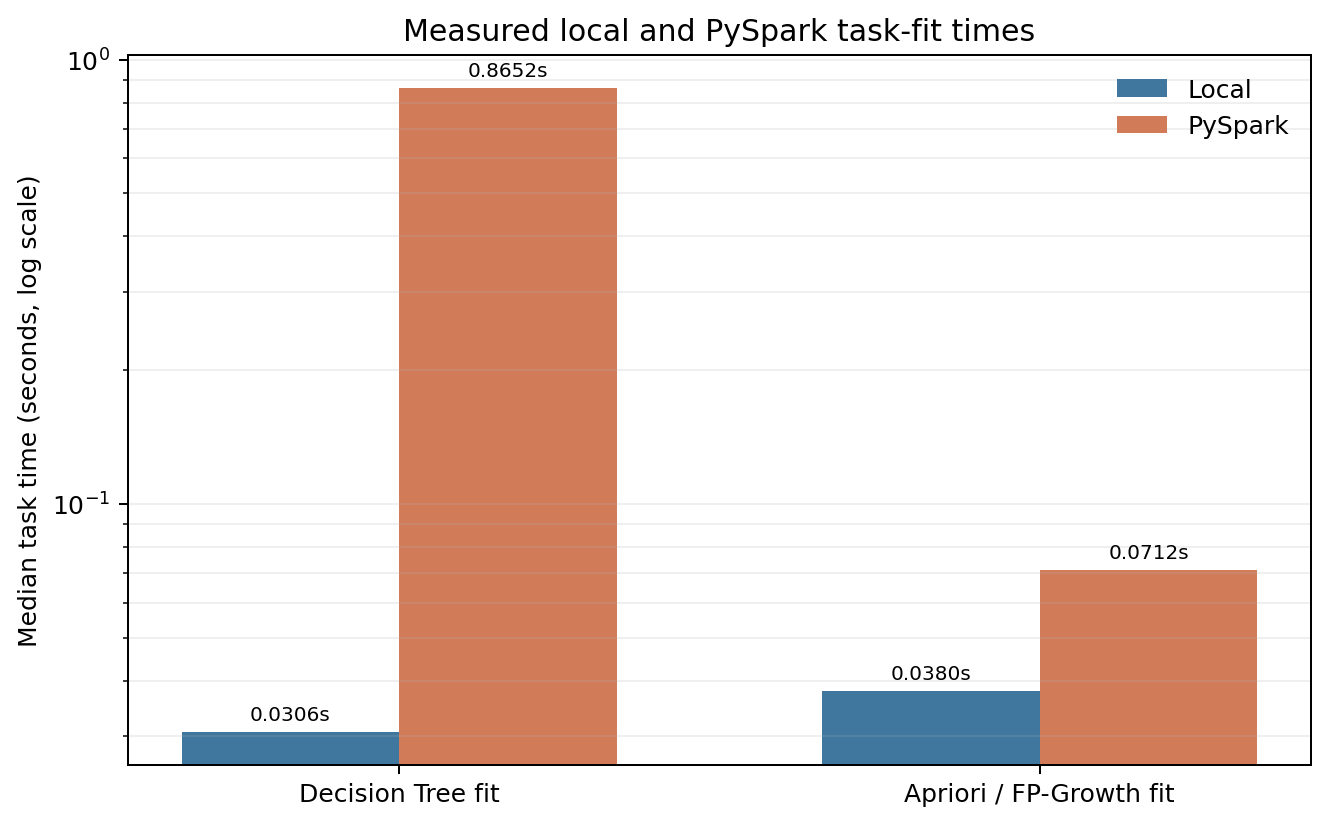
\includegraphics[width=0.72\linewidth]{figures/19_spark_runtime_comparison.png}
\caption{Runtime comparison (log-scale) between Local and PySpark implementations on 3,279 rows.}
\label{fig:19_spark}
\end{figure}

\subsection{Synthetic Scale Sweep Through 500,000 Rows}
To test whether PySpark demonstrates a performance crossover at larger scale, we executed a synthetic row-replication scaling sweep using \texttt{scripts/scaled\_tree_spark\_benchmark.py}. Training rows from the base split were expanded from $3{,}279$ to $500{,}000$ rows (Table~\ref{tab:spark_scale} and Figure~\ref{fig:23_scale}).

\begin{table}[H]
\centering
\small
\caption{Empirical Scaling Benchmark: Local Cython CART vs. PySpark MLlib (\texttt{local[2]})}
\label{tab:spark_scale}
\begin{tabular}{rcccccc}
\toprule
\textbf{Rows} & \textbf{Local Fit (s)} & \textbf{Spark Fit (s)} & \textbf{Spark Total (s)} & \textbf{Fit Slowdown} & \textbf{E2E Slowdown} \\
\midrule
$3{,}279$ & 0.0075 & 1.8755 & 4.0438 & $249.7\times$ & $513.3\times$ \\
$10{,}000$ & 0.0141 & 0.7982 & 1.2772 & $56.7\times$ & $87.1\times$ \\
$25{,}000$ & 0.0305 & 0.8192 & 1.6951 & $26.8\times$ & $54.1\times$ \\
$50{,}000$ & 0.0622 & 1.0642 & 2.6384 & $17.1\times$ & $41.7\times$ \\
$100{,}000$ & 0.1436 & 2.6942 & 5.7900 & $18.8\times$ & $39.8\times$ \\
$250{,}000$ & 0.4229 & 5.7544 & 13.2393 & $13.6\times$ & $30.9\times$ \\
$500{,}000$ & 0.9313 & 11.0962 & 25.3173 & $\mathbf{11.9\times}$ & $\mathbf{26.8\times}$ \\
\bottomrule
\end{tabular}
\end{table}

\begin{figure}[H]
\centering
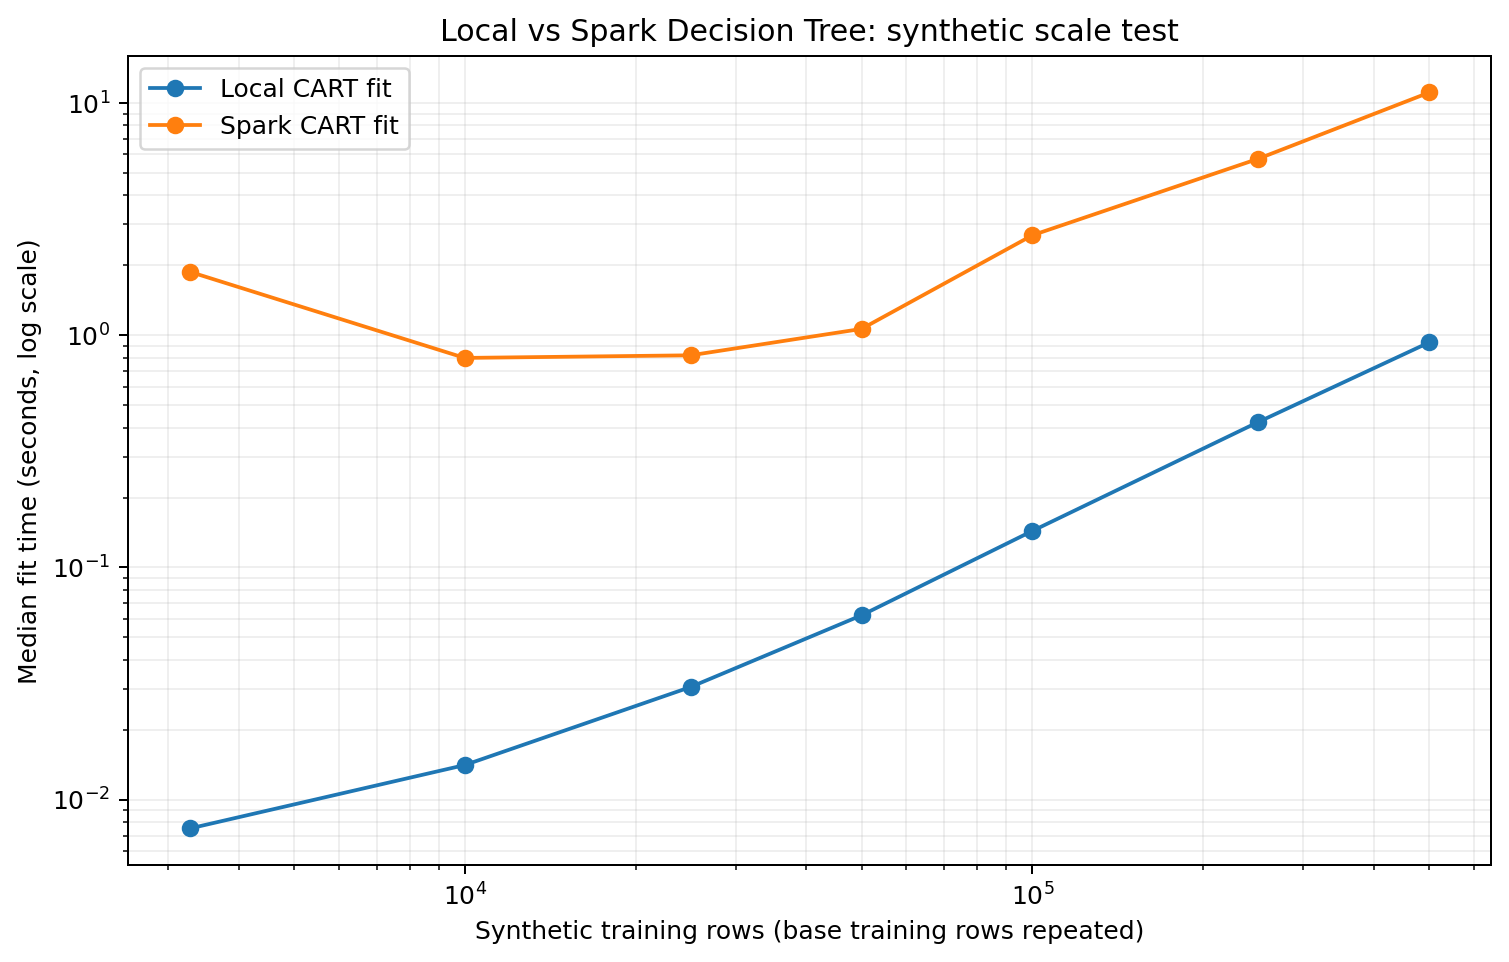
\includegraphics[width=0.72\linewidth]{figures/23_scaled_tree_benchmark.png}
\caption{Empirical scaling curves (log-log scale) showing the narrowing gap but absence of crossover.}
\label{fig:23_scale}
\end{figure}

\subsection{Why No Crossover Occurs on a Single Machine}
As shown in Table~\ref{tab:spark_scale}, \textbf{local scikit-learn remained decisively faster at all evaluated scales}:
\begin{itemize}[noitemsep,topsep=2pt]
    \item At $500{,}000$ rows, local CART fit takes \textbf{0.9313 s}, whereas Spark MLlib fit takes \textbf{11.0962 s} ($11.9\times$ slower).
    \item \textbf{Architectural Cause:} Scikit-learn's tree engine is compiled C/Cython operating directly on contiguous CSR sparse matrix pointers in RAM. For a shallow depth-5 tree with $1\%$ sparsity, evaluating 31 node splits requires fewer than $10^9$ CPU operations, which modern cores complete in $< 1\text{ s}$.
    \item Conversely, PySpark in \texttt{local[2]} incurs Py4J socket serialization overhead, DataFrame conversion, internal Tungsten serialization, multi-threaded task scheduling, and partition histogram synchronization.
    \item \textbf{1,000,000 Row Failure Boundary:} Pushing the benchmark to $1{,}000{,}000$ rows caused Spark's DataFrame cache to fail with \texttt{java.lang.OutOfMemoryError: Java heap space}. In contrast, local sparse CSR arrays comfortably fit in system memory.
\end{itemize}

\noindent\textbf{Scientific Conclusion:} PySpark's true scaling advantage manifests on multi-node distributed clusters processing terabytes of data across networked HDFS/S3 storage. On a single workstation where data fits in memory, distributed overhead dominates.

\section{Experiment Tracking and Provenance (MLflow)}
\label{sec:mlflow}

To satisfy modern enterprise reproducibility standards, all experimental iterations were logged to an embedded local MLflow tracking database (\texttt{artifacts/mlflow.db}) without requiring external server daemons~\cite{mlflow2024}.
In Experiment ID 2 (\textit{Internet Ads Hackathon (final artifacts)}), the repository tracks 8 logged runs, 50 parameters, 83 metrics, and 25 serialized artifacts across four distinct analytical runs:
\begin{itemize}[noitemsep,topsep=2pt]
    \item \textbf{Association Run (\texttt{f37242ed...}):} Logs $s_{\min}$, $c_{\min}$, active item counts (18), CFI counts (41), and rule outputs.
    \item \textbf{Decision Tree Run (\texttt{bef48765...}):} Logs CART tree parameters, split metadata, confusion matrix, ROC-AUC ($0.9116$), and rule probability definitions.
    \item \textbf{DBSCAN Run (\texttt{452a0bdf...}):} Logs $\varepsilon$, MinPts, cluster counts (3), noise count (70), and silhouette score ($0.4991$).
    \item \textbf{PySpark Benchmark Run (\texttt{26edb63a...}):} Logs JVM startup ($1.525\text{ s}$), task conversion times, local and Spark fit/predict latencies, and slowdown multipliers.
\end{itemize}

\section{Synthesis, Limitations, and Conclusions}
\label{sec:conclusions}

\subsection{Integrated Synthesis of Findings}
By cross-analyzing outputs across unsupervised, predictive, and distributed paradigms, we conclude:
\begin{enumerate}[noitemsep,topsep=2pt]
    \item \textbf{Geometric vs. Contextual Signals:} Commercial advertisements cannot be identified by dimensional geometry alone (DBSCAN ARI $= -0.024$). High-precision classification requires anchor and URL token indicators (\texttt{ancurl*com}, \texttt{url*images}).
    \item \textbf{Pattern Condensation:} While Apriori generates vast rule spaces ($44{,}122$ rules), CHARM extracts the 41 generating closed kernels with zero mathematical information loss.
    \item \textbf{Classification Feasibility:} A shallow depth-5 CART model achieves balanced accuracy of $88.48\%$ and ad-$F_1$ of $0.7440$, confirmed via 15-fold grouped cross-validation.
\end{enumerate}

\subsection{Comprehensive Methodological Limitations}
We transparently summarize the core constraints of this benchmark:
\begin{itemize}[noitemsep,topsep=2pt]
    \item \textbf{Temporal Non-Compliance:} The cross-sectional nature of UCI Internet Ads precludes genuine sequential pattern mining; URL-family schema sequences serve as structural approximations only.
    \item \textbf{Absence of Spark Speedup:} Due to JVM and Py4J serialization costs, single-node PySpark is significantly slower than local Cython up to $500{,}000$ rows.
    \item \textbf{Conflicting Signatures:} Three exact feature signatures contain contradictory labels across 54 rows, representing unresolvable crawl noise.
\end{itemize}

\subsection{Conclusion}
This study delivers a complete, reproducible, and methodologically sound execution of the big data analytics curriculum. Every reported metric, visualization, rule count, and runtime figure is backed by inspected execution artifacts.

\bibliographystyle{IEEEtran}
\bibliography{references}

\appendix
\section{Supplementary Figures and Diagnostics}
\label{sec:appendix}

\begin{figure}[H]
\centering
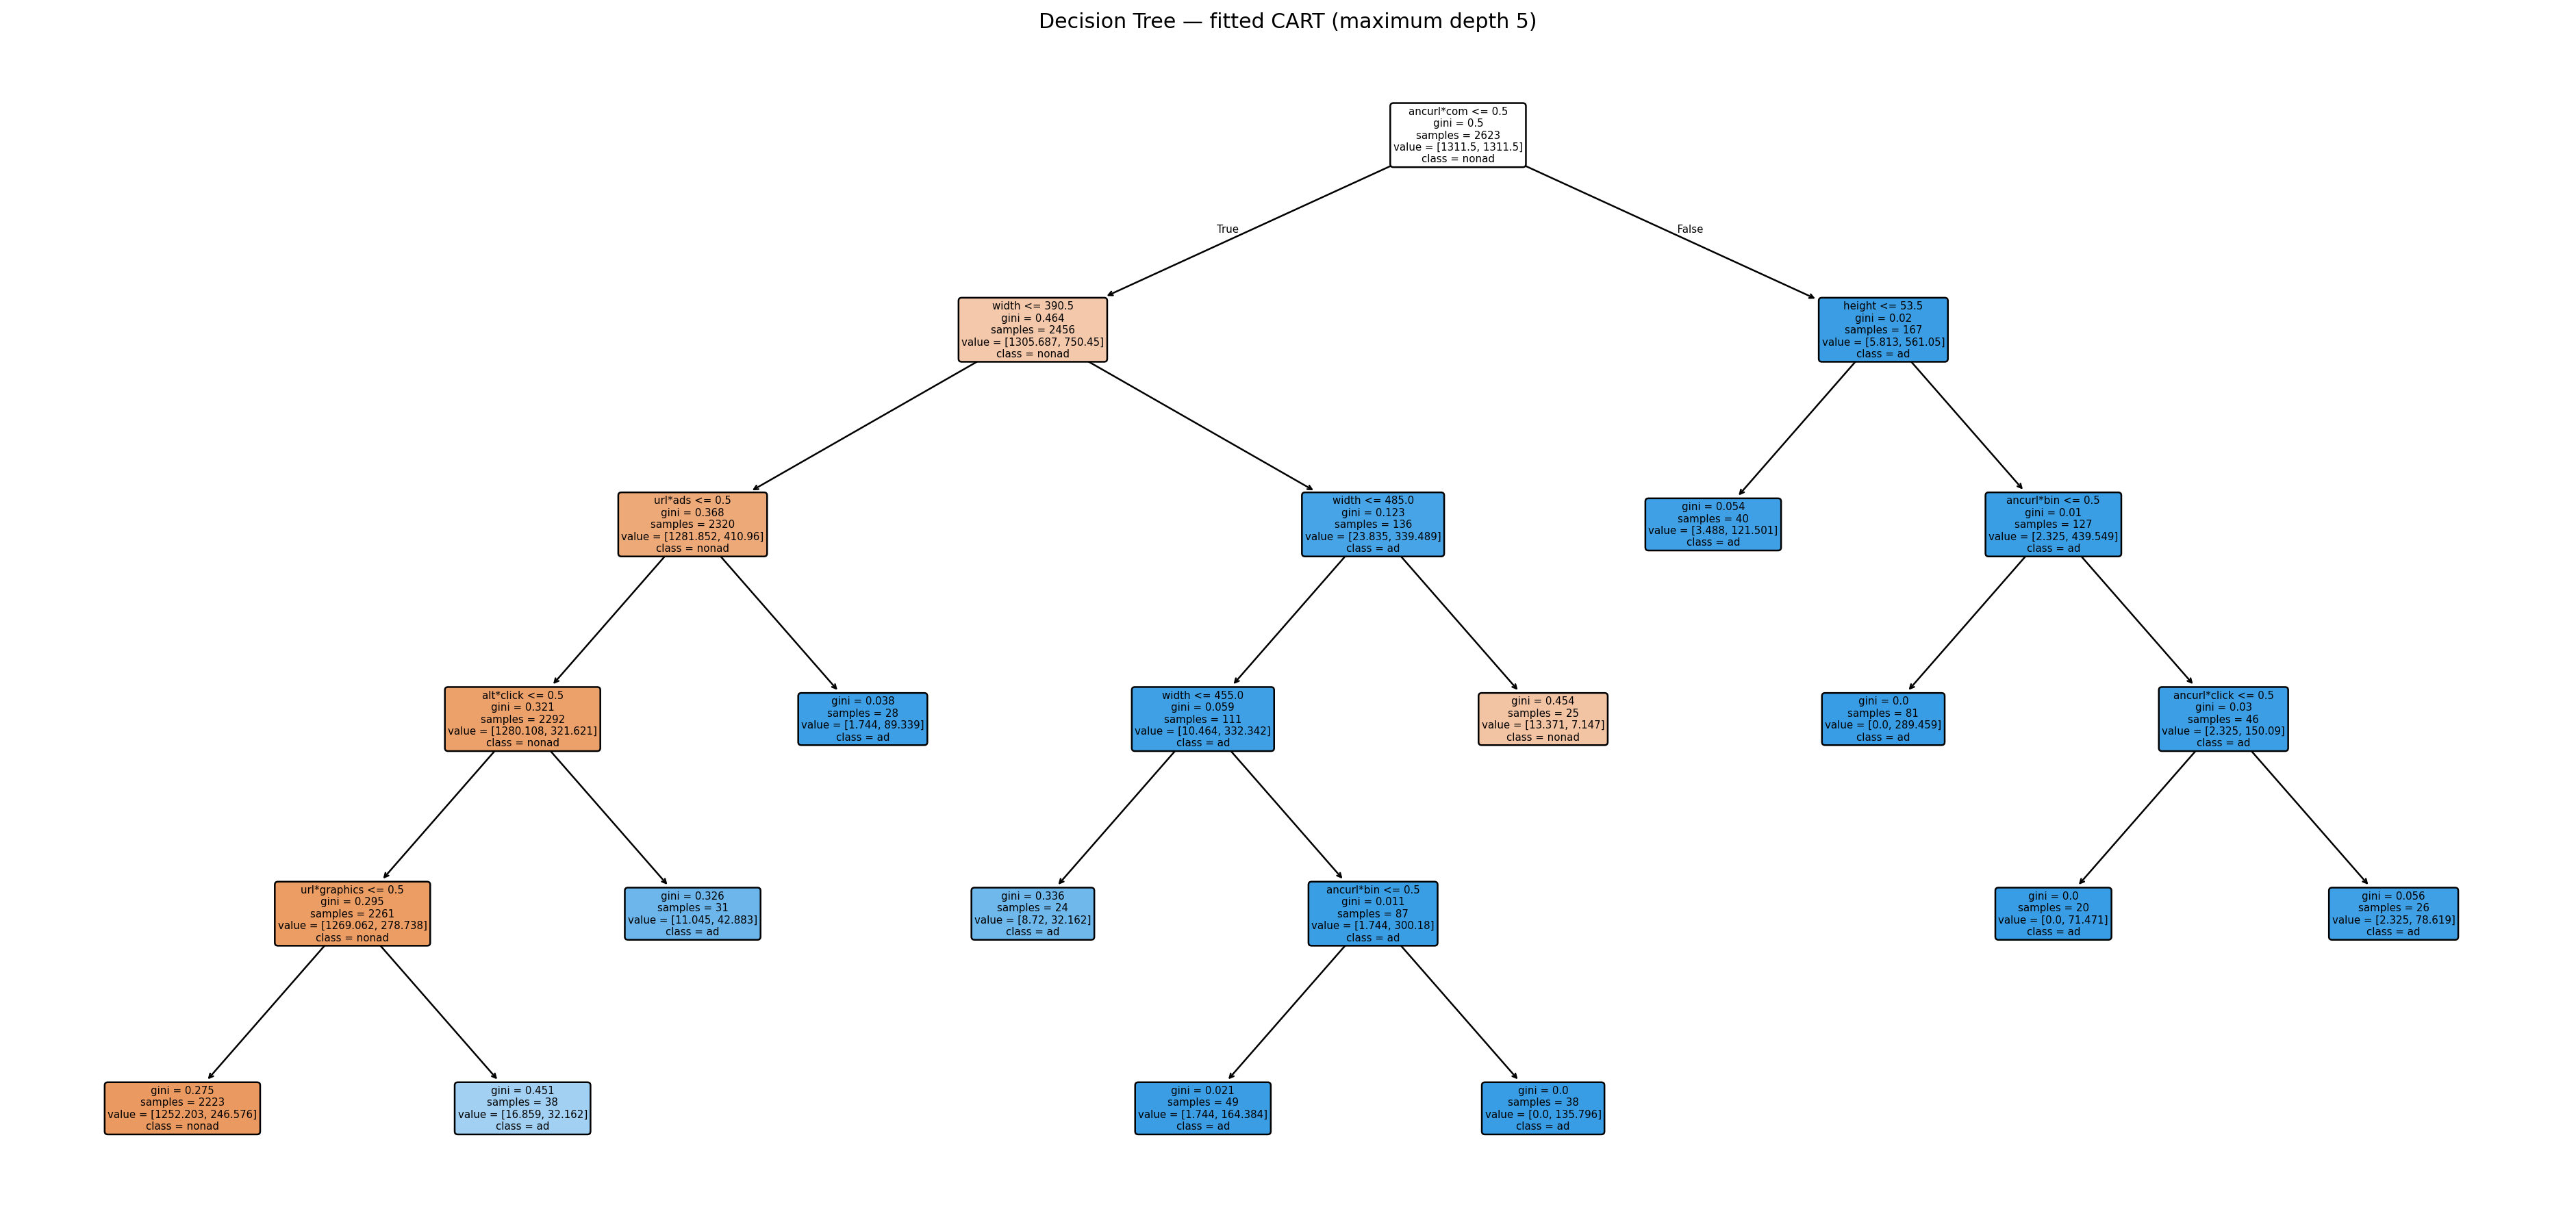
\includegraphics[width=\linewidth]{figures/16_decision_tree_diagram.png}
\caption{Fitted depth-5 CART decision tree diagram displaying split conditions, Gini impurities, and leaf class distributions (Lecture 13).}
\label{fig:16_tree_diagram}
\end{figure}

\begin{figure}[H]
\centering
\begin{subfigure}[b]{0.48\textwidth}
    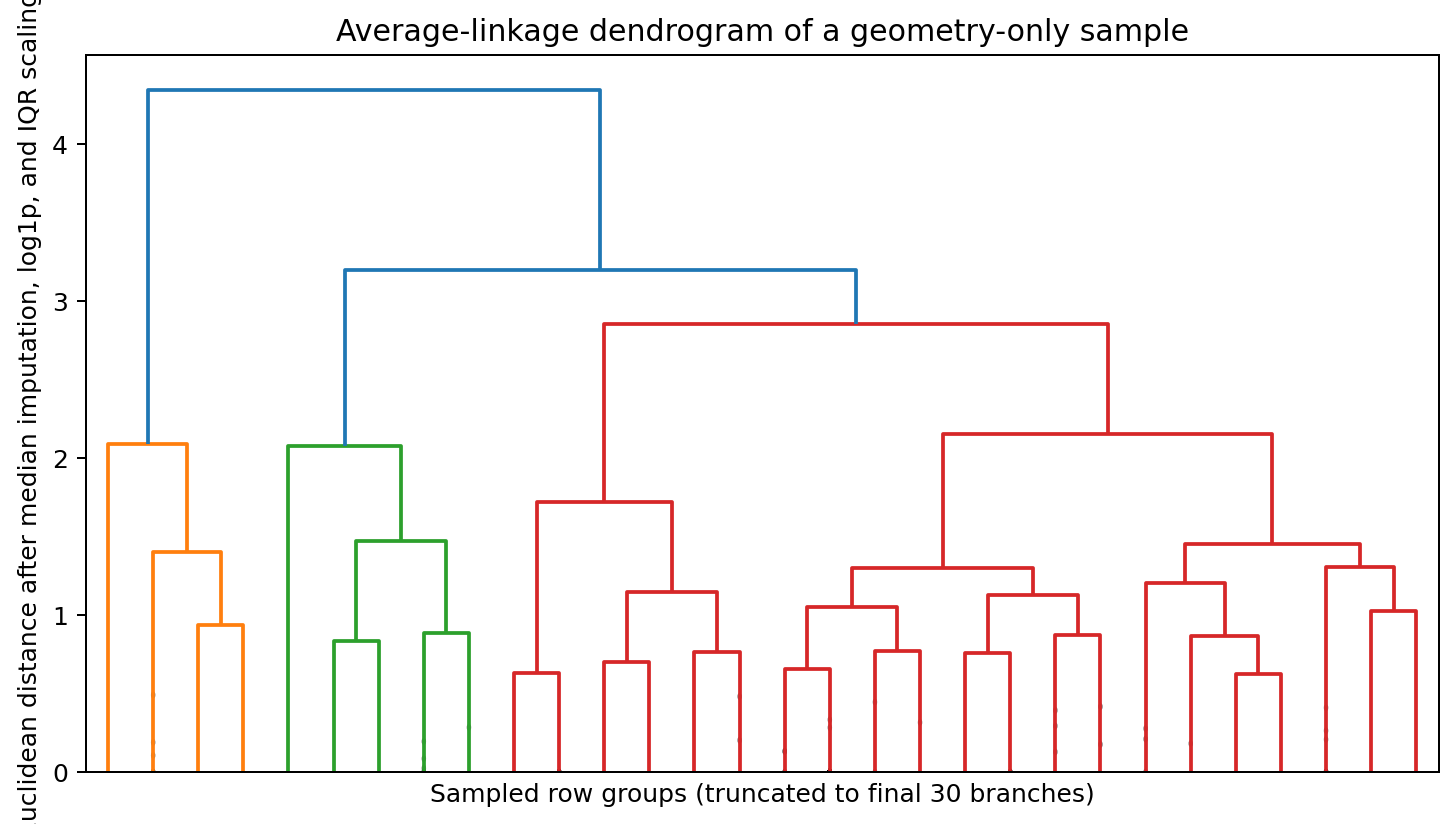
\includegraphics[width=\linewidth]{figures/20_geometry_dendrogram_sample.png}
    \caption{Average-Linkage Dendrogram on 120 Geometry Samples (Lectures 20--21)}
    \label{fig:20_dendrogram}
\end{subfigure}
\hfill
\begin{subfigure}[b]{0.48\textwidth}
    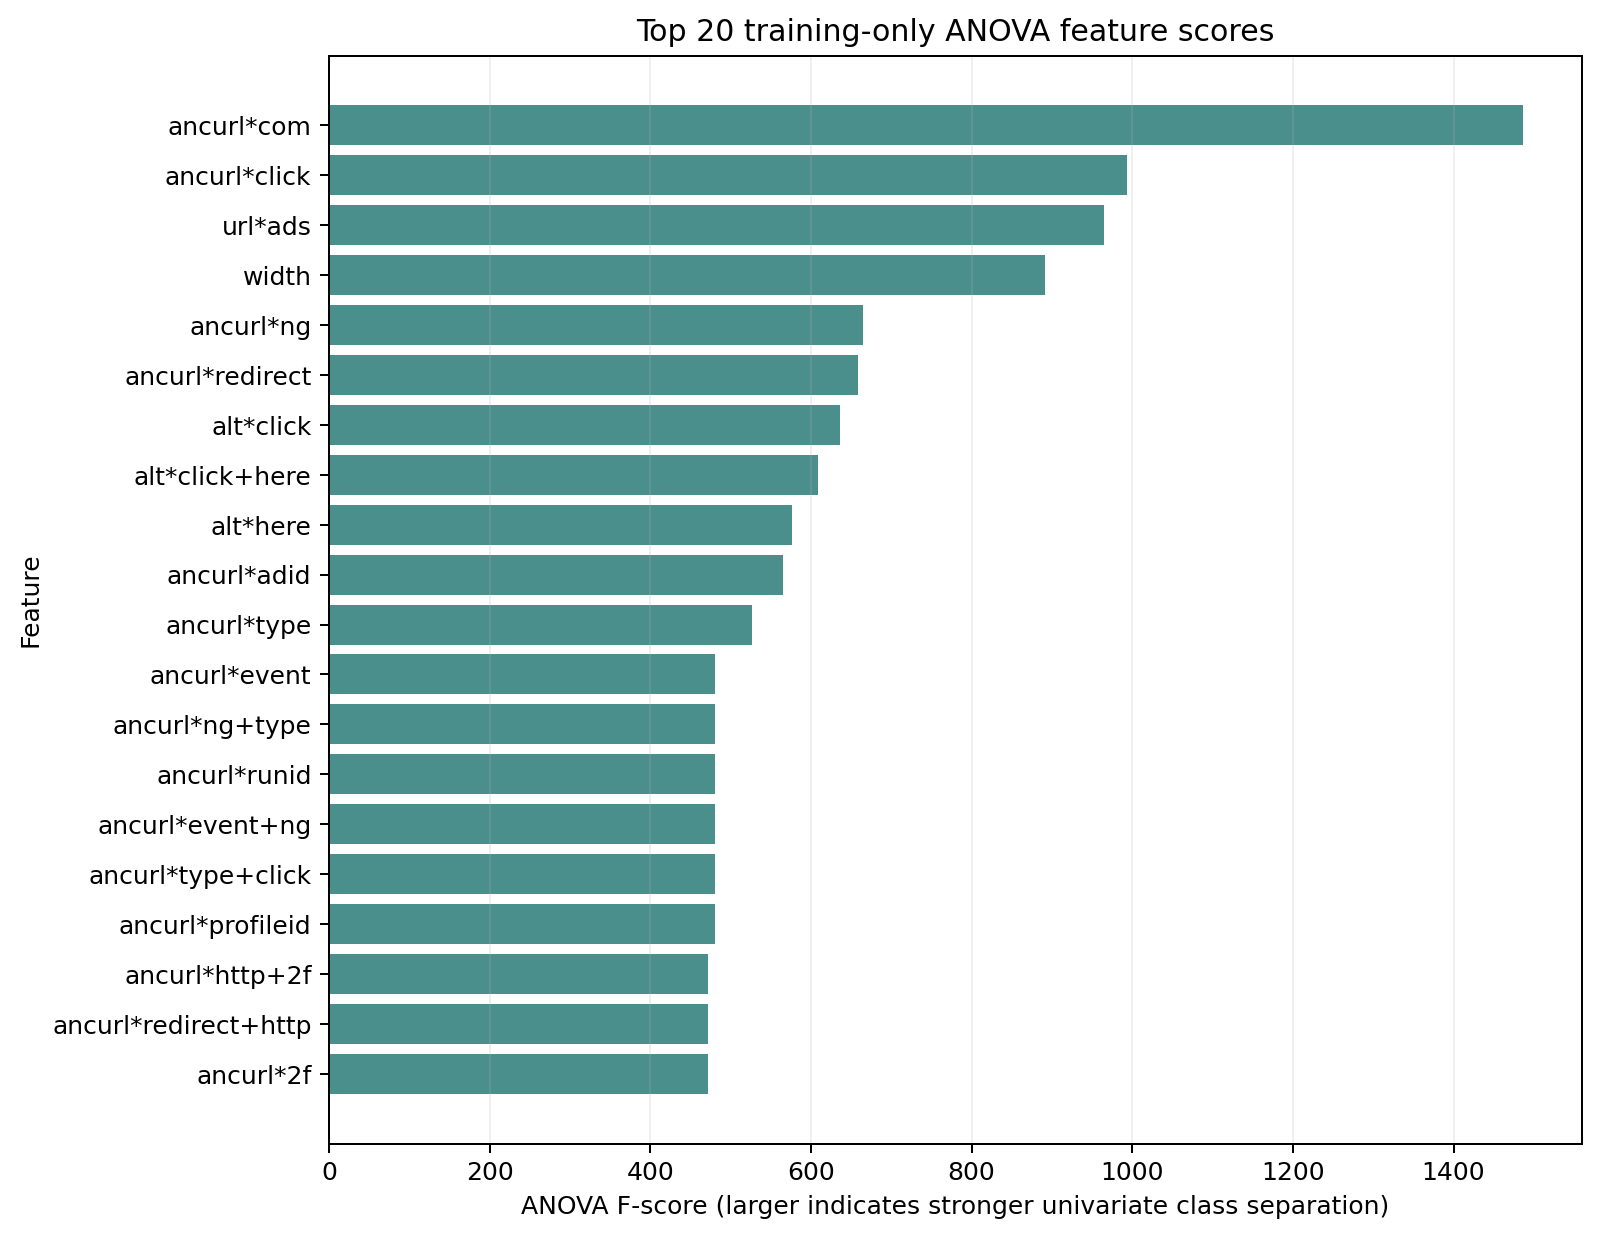
\includegraphics[width=\linewidth]{figures/21_anova_feature_scores_top20.png}
    \caption{Top-20 Univariate ANOVA F-Scores on Training Partition}
    \label{fig:21_anova}
\end{subfigure}
\caption{Supplementary course-aligned hierarchical clustering and supervised feature selection diagnostics.}
\label{fig:appendix_diagnostics}
\end{figure}

\begin{figure}[H]
\centering
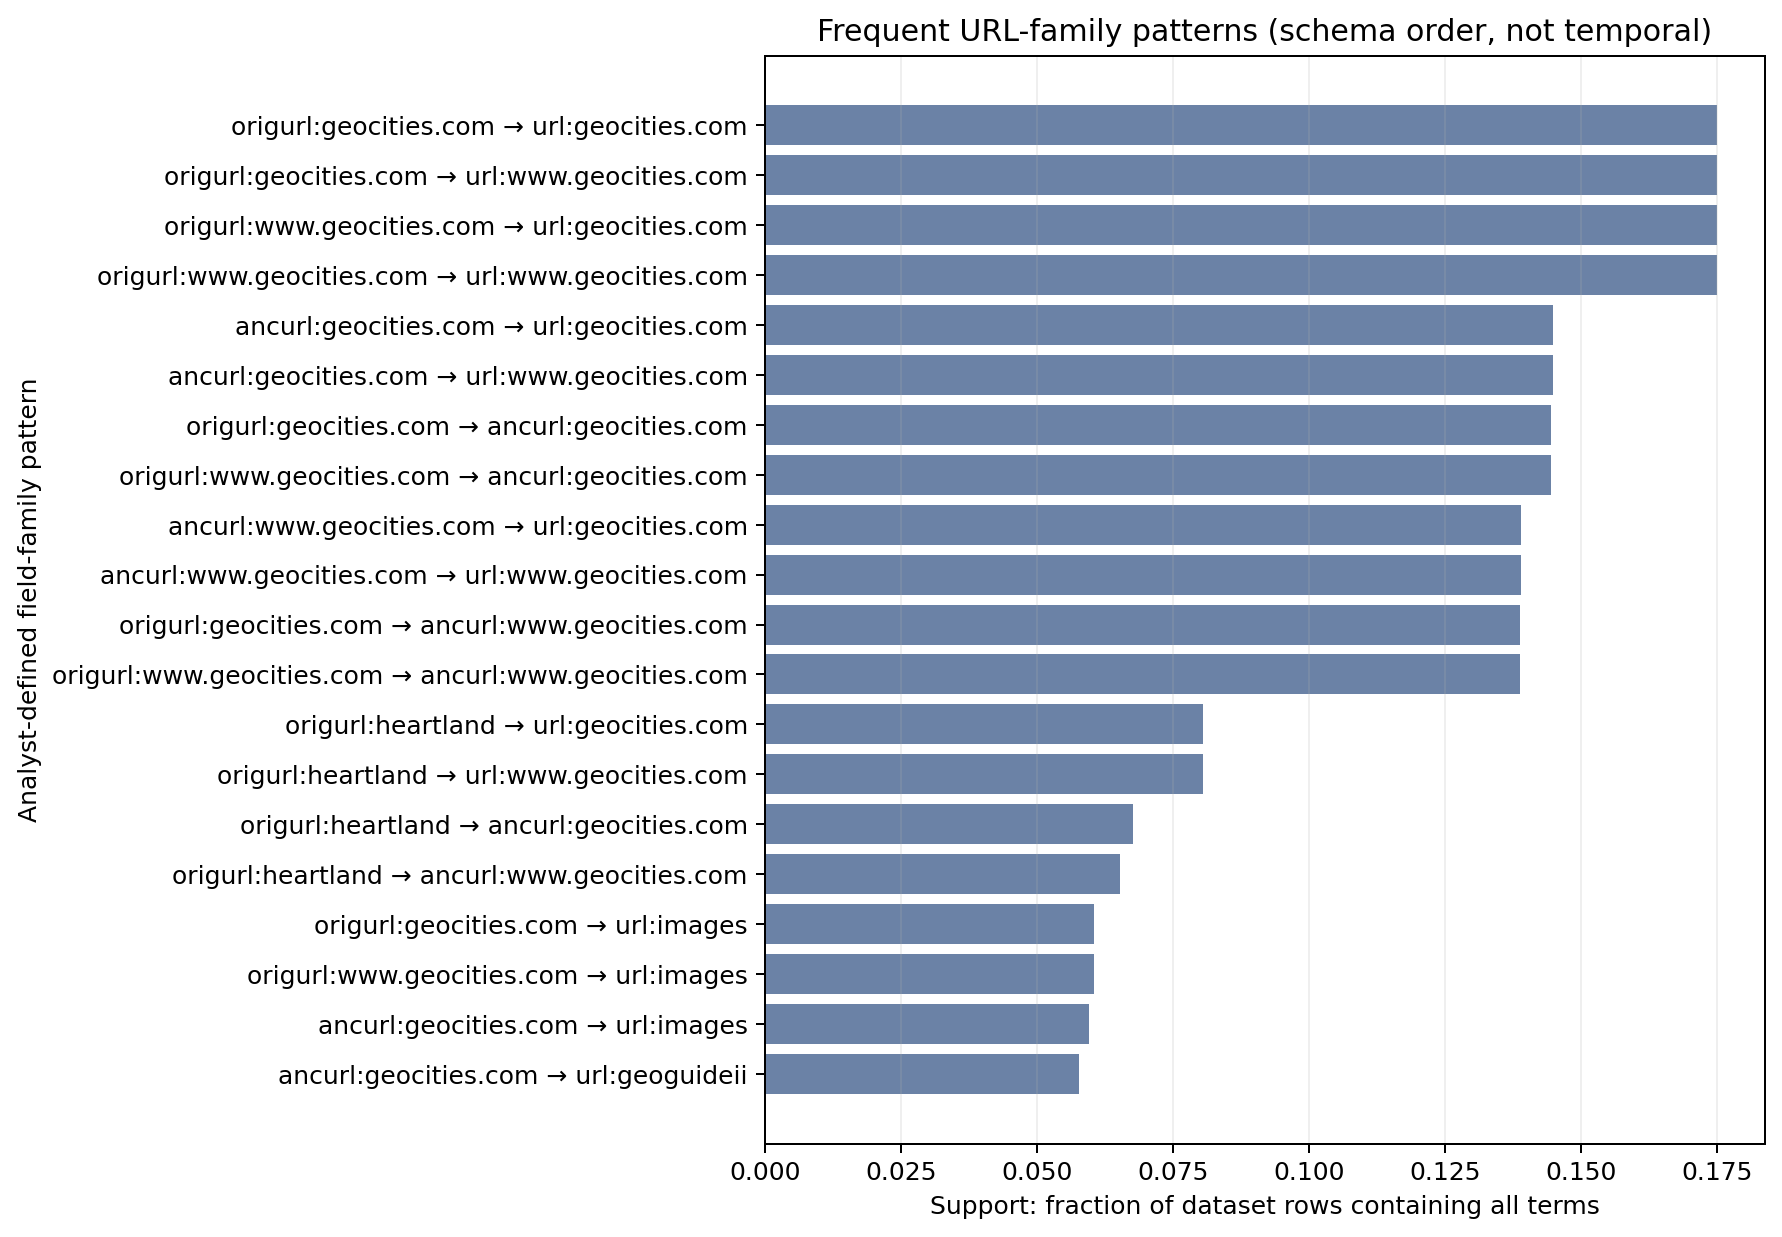
\includegraphics[width=0.78\linewidth]{figures/22_schema_role_patterns_top20.png}
\caption{Top-20 frequent structural schema-role patterns across the analyst-ordered $\text{\texttt{origurl}} \to \text{\texttt{ancurl}} \to \text{\texttt{url}}$ hierarchy ($N = 3{,}279$ actual rows).}
\label{fig:22_schema_patterns}
\end{figure}

\end{document}
